\documentclass[11pt,notitlepage,a4paper]{article}

\usepackage[left=3.7cm,right=3.7cm,top=3cm,bottom=3cm]{geometry}
\usepackage{graphicx}
%%BeginIpePreamble
\usepackage{amssymb,mathtools, amsmath, amsfonts, amsthm}
%%EndIpePreamble
%\usepackage{color}
\usepackage{float}
\usepackage{hyperref}
\usepackage{enumerate}
\usepackage{enumitem}
\usepackage{chngcntr}
\usepackage{cleveref}
\usepackage{pdfpages}

\counterwithout{equation}{section}



\newlength{\margen}
\setlength{\margen}{\paperwidth}
\addtolength{\margen}{-\textwidth}
\addtolength{\skip\footins}{0.7 cm}
\setlength{\margen}{0.5\margen}
\addtolength{\margen}{-1in}
\setlength{\oddsidemargin}{\margen}
\setlength{\evensidemargin}{\margen}
\setlength{\abovedisplayskip}{3pt}
\setlength{\belowdisplayskip}{3pt}
%%%% Small setup %%%%
\hypersetup{
	colorlinks=false,
	pdfborder={1 1 0.0005},
}
\setlength{\parskip}{0.2cm}
%%%%%%%%%%%%%%%
\usepackage{tikz-cd}
\usetikzlibrary{cd}
\usepackage[english]{babel}
\usepackage{todonotes}
\usepackage{cleveref}
\usepackage{caption}
\usepackage{subcaption}
\usepackage{bbding}
\usepackage{tcolorbox}
\usepackage{natbib}

\DeclareMathOperator{\incl}{incl}

\newtheorem{proposition}{Proposition}[section]
\newtheorem{fact}{Fact}[section]
\newtheorem{theorem}{Theorem}[section]
\newtheorem{lemma}{Lemma}[section]
\newtheorem{corollary}{Corollary}[section]
\theoremstyle{definition}
\newtheorem{definition}{Definition}[section]
\newtheorem{propdef}{Proposition / Definition}[section]
\newtheorem{remark}{Remark}[section]

\newtheorem{inneraxiom}{Axiom}
\newenvironment{axiom}[1]
{\renewcommand\theinneraxiom{#1}\inneraxiom}
{\endinneraxiom}
\newcommand{\cc}{\mathfrak{c}}
\newcommand{\Z}{\mathbb{Z}}
\newcommand{\CC}{\mathbb{C}}
\newcommand{\Q}{\mathbb{Q}}
\newcommand{\R}{\mathbb{R}}
\newcommand{\N}{\mathbb{N}}
\newcommand{\Hc}{\mathcal{H}}
\newcommand{\Lan}{\mathcal{L}}
\newcommand{\Ln}{\lim\limits_{n\to \infty}}
\newcommand{\clist}{\mathfrak{c}_{1}, \cdots, \mathfrak{c}_m}
\newcommand{\morph}[1]{\stackrel{#1}{\simeq}}
\newcommand{\vlst}[2]{#1_1,\dots, #1_{#2}}
\newcommand{\gnp}{G(n,\beta_1/n^{a_1-1}, \dots,\beta_l/n^{a_l-1})}



\begin{document}
	
	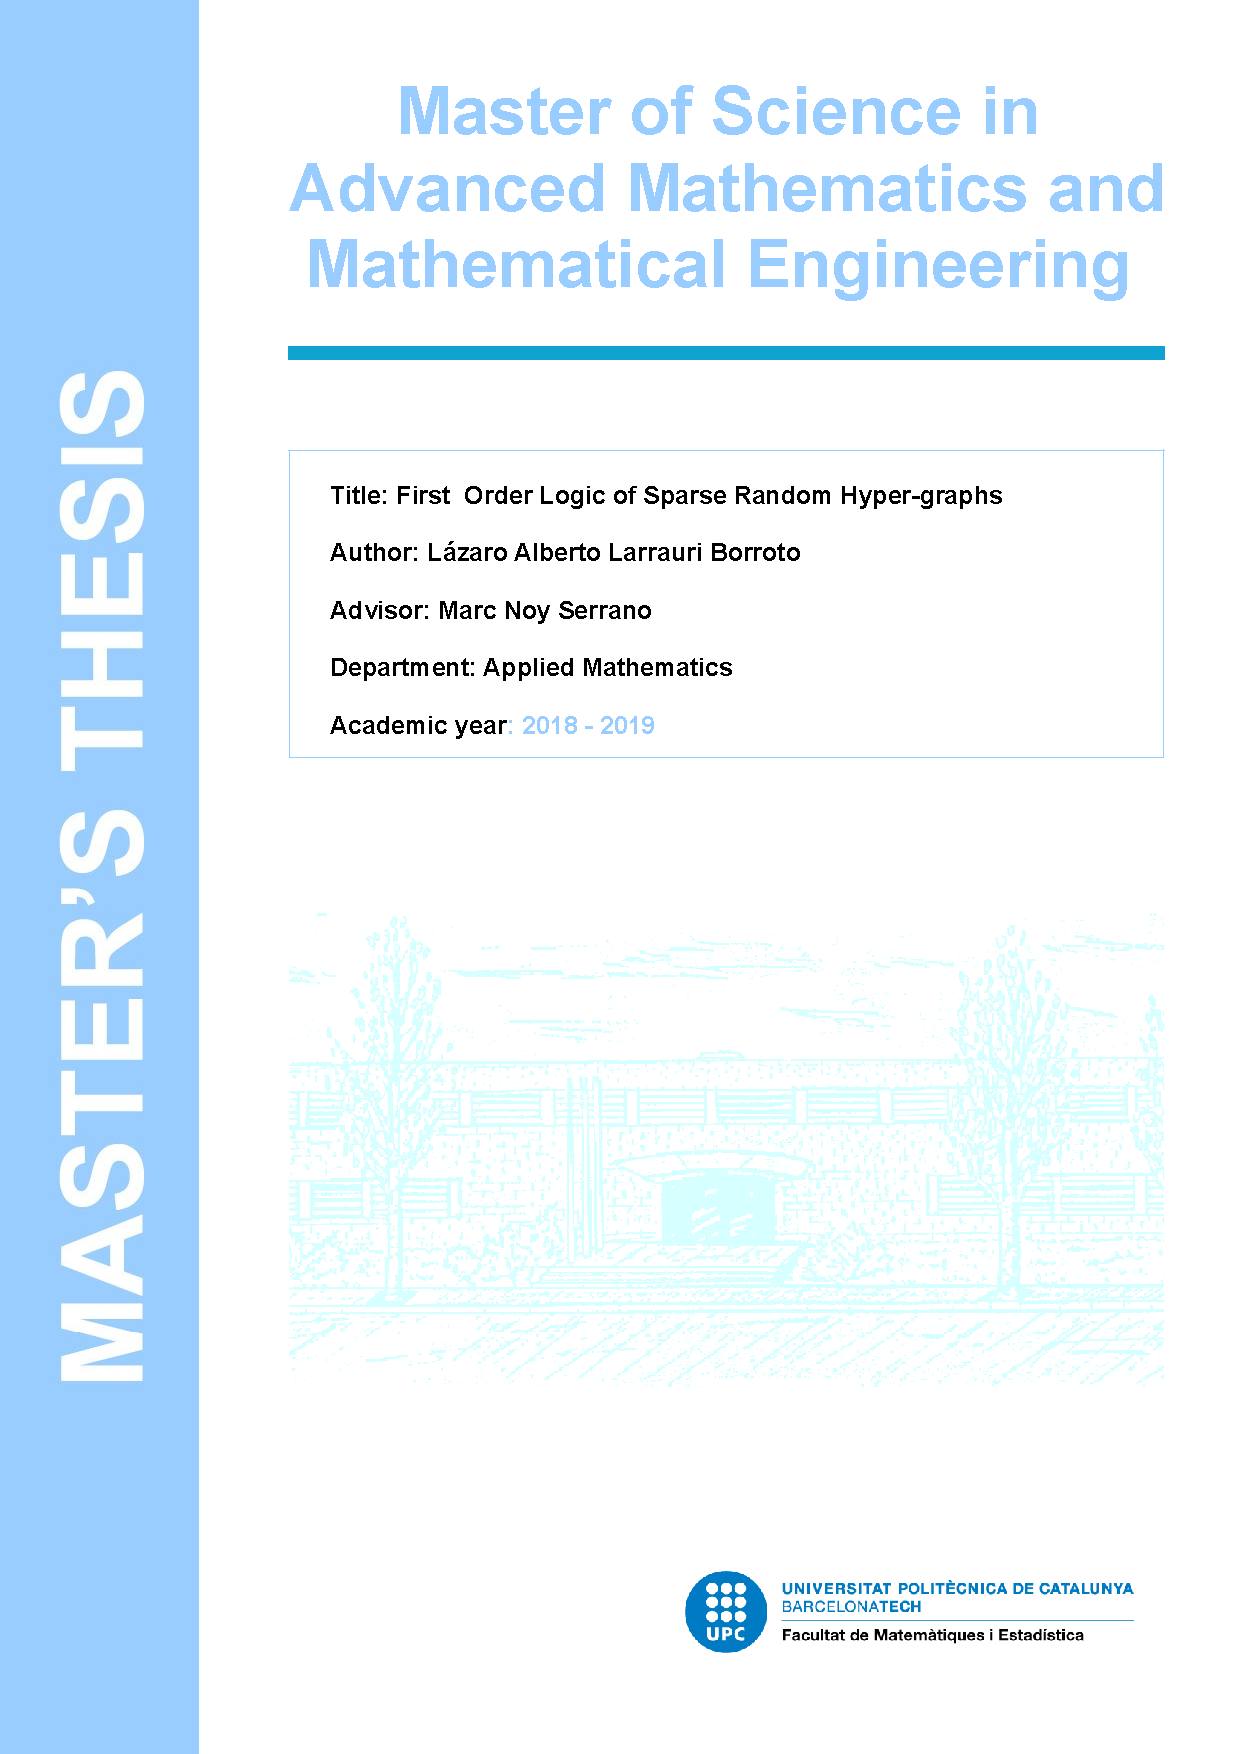
\includepdf{Portada.pdf}
	
\begin{abstract}
	We give a generalization the results from Lynch in \cite{lynch1992probabilities}
	on the convergence law for sparse random graphs to sparse random hypergraphs.
\end{abstract}
\clearpage
\tableofcontents
\clearpage

\section*{Introduction}

This work is the thesis presented for the Master in Applied Mathematics and 
Mathematical Engineering of the Universitat Politècnica de Catalunya in 
June 2019. \par

This text belongs to the study of the asymptotic properties of random structures.
This is an active area of mathematics that has gained recent popularity due to 
the increasing need for methods that allow for analysis of large random
structures. These structures appear in a wide array of 
``real-life" problems, ranging
from the study of social networks to biology, and they are
arguably interesting in their own right.\par

The objective of this work, proposed by Marc Noy and Albert Atserias, was 
to generalize the results obtained in \cite{lynch1992probabilities} to more
general random structures. This was motivated by applications to the study
of the satisfability of random CNF formulas, but those are out of the scope of 
this work. \par

Going into further detail, in \cite{lynch1992probabilities} the asymptotic 
behavior under first order logic of the Erdös-Rényi binomial model $\mathcal{G}(n,p)$, where
$p$ is taken as a decreasing function on $n$ of the form $\beta\cdot n^{-1}$,
is studied. The first order properties of graphs are the ones expressible in 
terms of quantification over vertices and Boolean combinations of statements 
of the form ``$x$ adjacent to $y$'' and  ``$x$ equal to $y$''. The main theorem
in \cite{lynch1992probabilities} states that the limit probability that a graph
in $\mathcal{G}(n,\beta/n)$ satisfies any given first-order property exists
and has good properties with respect to $\beta$. \par


The original goal was to give a generalization for the case of uniform hypergraphs
but the techniques used for that case also allowed for a generalization for 
hypergraphs with multiple edge sets of different sizes.  

\clearpage




\section{Logic of Sparse Random Graphs}

We give a brief overview of \cite{lynch1992probabilities}.
The asymptotic behavior of graphs in $G(n,\beta/n)$ is as follows
	\begin{itemize}
	\item The number of cycles of 
	length $3,4\dots, r$
	are asymptotically distributed like independent Poisson 
	variables.
	\item Small cycles are a.a.s (asymptotically almost surely) far away.
	\item Fixed vertices are a.a.s far away.
	\item The ball of a given radius centered in fixed
	vertex is a.a.s a tree. Any tree occurs with a positive 
	probability.
\end{itemize}

This way, asymptotically, trees of any kind occur arbitrarily often in a typical
random graph. Given the locality of first order logic up to a fixed 
quantifier rank this is tells us that the only way 
to distinguish large random graphs in $G(n,\beta/n)$ under first order logic
(up to a fixed quantifier rank) 
is by looking at the neighborhoods of their small cycles. \par

It is given a finite and exhaustive classification of the uni-cyclic
graphs with less than a given radius. After that it is shown that
if two graphs $G_1$ and $G_2$ contain the same number 
of uni-cycles of each type or they
contain a large enough number of those then they are a.a.s equivalent
under first order logic up to some quantifier rank $k$. This is done by giving
a winning strategy for duplicator in the Ehrenfeucht Fraisse game of $k$ rounds played on 
$G_1$ and $G_2$.\par

Finally it is shown that the quantities of uni-cycles of each type in a random graph
are asymptotically distributed like independent Poisson variables 
whose means are given by some other nested ``Poisson expressions" that correspond 
to the trees hanging from each uni-cycle. 



%In this chapter we will review the results obtained
% in the paper with the same name by James F. Lynch \cite{lynch1992probabilities}.
%In there, limit probabilities of sentences in the first order language of graphs $\mathcal{L}$
%are discussed for the binomial model $G(n,p)$ in the cases $p=\beta/n$ and
%$p=\beta n^{-\alpha}$ with $\alpha=(l+1)/l$ . \par
%
%More precisely, it is proven that in those cases the 
%probability of every sentence converges and it is shown
%that for any of those sentences, its limit probability 
%is among the values taken by some analytic formulas
%with parameter $\beta$. \par
%
%We are interested in the case $p=\frac{\beta}{n}$, which is 
%the one discussed more extensively in \cite{lynch1992probabilities}. 
%According to the author, the relevant theorems for 
%the other case can be proven analogously. From now on we
%will only refer as random graphs to the ones in $G(n,\beta/n)$\par
%
%From now on we will denote by $\mathrm{Poiss}_\lambda$ the probability
%function of the Poisson distribution with mean $\lambda$.
%That is, the one given by $\mathrm{Poiss}_\lambda(n)=e^{-\lambda}\lambda^n/n!$ 
%for any $n\in \N$.
%Also, we define $\mathrm{Poiss}_\lambda(\leq n)$ and $\mathrm{Poiss}_\lambda(>n)$ as 
%$\sum_{i=0}^n \mathrm{Poiss}_\lambda(n)$ and $1-\mathrm{Poiss}_\lambda(\leq n)$
%respectively. Notice that for a fixed $n$, both $\mathrm{Poiss}_\lambda(\leq n)$ 
%and $\mathrm{Poiss}_\lambda(>n)$ can be considered real functions of parameter $\lambda$. \par
%
%We define the following sets of functions. Let $\Lambda$ be the smallest 
%set of expressions with parameter $\beta$ such that:
%
%\begin{itemize}[noitemsep, topsep=0pt]
%	\item $1\in \Lambda$,
%	\item For any $\lambda \in \Lambda$ and $i\in \N$, 
%	both $\mathrm{Poiss}_{\beta\lambda}(n)$ and $\mathrm{Poiss}_{\beta\lambda}(> n)$ are in
%	$\Lambda$.
%	\item For any $\lambda_1,\lambda_2 \in \Lambda$,
%	$\lambda_1 \lambda_2$ belongs to $\Lambda$ as well.
%\end{itemize}
%
%And let $\Theta$ be the smallest set of functions with parameter $\beta$
%such that:
%\begin{itemize}[noitemsep, topsep=0pt]
%	\item For any $\lambda \in \Lambda$ 
%	and $n,a,i\in \N$, with $i\geq 3$, 
%	both $\mathrm{Poiss}_{\beta^i\lambda/a}(\leq n)$ and $\mathrm{Poiss}_{\beta^i\lambda/a}(> n)$
%	are in $\Theta$.
%\end{itemize} 
%
%The main result is the following:
%
%\begin{theorem}[Lynch, 1992] \label{thrm:main}
%	Let $\phi$ be a sentence in the first order theory of graphs. Then the limit
%	$\lim\limits_{n\to \infty} P(G(n,\beta/n) \models \phi )$ exists for all positive real numbers
%	$\beta$, and it is a finite sum of expressions in $\Theta$.
%\end{theorem}
%
%We show now an outline of the proof. \par 
%We show that for any quantifier rank $k$ there are some classes of graphs 
%$C^k_1,\dots, C^k_{n_k}$ such that
%\begin{itemize}[noitemsep, topsep=0pt]
%	\item[(1)] a.a.s the rank $k$ type of any two graphs in the same class coincide, 
%	\item[(2)] a.a.s. any random graph belongs to some of them, and
%	\item[(3)] the limit probability of random graph belonging to any of them is an expression in $\Theta$. 
%\end{itemize}
%
%After this is archived the theorem follows easily. Indeed, let $\phi$ be a sentence 
%in the first order language $\Lan$ of graphs whose quantifier rank is $k$, and denote by
%$G$ a random graph in $G(n,\beta/n)$. \par
%
%The objective of next sections will be to define the classes $C_1,\dots, C_{n_k}$ and to show
%that they satisfy properties (1), (2) and (3). Later we will prove a stronger result, so we will
%allow ourselves to just sketch some of the proofs during this chapter. 
%
%\section{Agreeability Classes}
%
%
%It is known that $n^{-v/e}$ is the t
%hreshold probability for the appearance 
%of a balanced graph of density $v/e$. 
%In our case $v/e=1$, so in consequence any connected graph $H$
%with $e(H)< v(H)$ a.a.s will not appear 
%as a subgraphs of $G(n,\beta/n)$. It can be easily 
%shown that such graphs $H$ are exactly 
%the ones containing more than one cycle. \par
%
%If $H$ is a connected graph with $v=e$, then $H$ is an uni-cyclic graph.
%In this case, the number $X_H$ of copies of $H$ 
%in $G(n,\beta/n)$ will asymptotically have non-zero bounded expectancy $m$. 
%It does not take much work to prove, using Brun's sieve, 
%that $X_H$ converges in distribution to a Poisson 
%random variable with mean $m$ as $n$ goes to infinity.  \par
%
%Finally, if $H$ is a connected graph 
%with $v>e$ then it must be a tree. Here 
%the expected number of copies of $H$ 
%in $G(n,\beta/n)$ diverges asymptotically. 
%Informally, trees of any kind will occur arbitrarily often. \par
%
%This all means, in a sense, that a.a.s the only 
%difference between large graphs in $G(n,\beta/n)$
%lies in their uni-cyclic subgraphs. More precisely,
%because of the ``locality" of first order logic of quantifier 
%rank $k$ we will only be interested in the 
%``small`` neighborhoods of the ``short" cycles.  
%Thus, our goal will be to classify uni-cyclic graphs
%in a way that respects equivalence under first 
%order logic of quantifier rank $k$. \par
%~\par
%To make our classification suitable for proofs 
%involving E.F. games we need to work graphs to which we ``attach" labels. 
%We define the set of symbols $Const=\{c_i\}_{i\in \N}$ 
%as the set of constants. Also, we will denote by
%$Const_n$ the set $\{c_1,\dots, c_n\}$.
% 
%\begin{definition} 
%	A \textbf{co-labeling} of a graph $G=(V,E)$ is a map 
%	$\sigma: D\rightarrow V$, where $D\subset C$ is a 
%	finite set of constant symbols. Given $c_i\in D$, 
%	we will say that the vertex $\sigma(c_i)$ is labeled $c_i$.
%	Equivalently, we can denote a labeling $\sigma$ as a tuple
%	$(c_{i_1}[x_1],\dots, c_{i_m}[x_m])$ where each $c_{i_j}$
%	 is a constant symbol, and $x_j$ is the vertex
%	in $V$ labeled $c_{i_j}$.
%\end{definition}
%
%\begin{definition} 
%	A \textbf{graph with constants}\footnote{
%		Compare with \cite{lynch1992probabilities}, where they are called ``rooted graphs". 
%		}
%	$G(c_{i_1}[x_1],\dots, c_{i_m}[x_m])$ 
%	is a graph $G$ together with a co-labeling 
%	$(c_{i_1}[x_1],\dots, c_{i_m}[x_m])$. 
%\end{definition}
%
%To keep our notation compact we will often drop 
%he $x_i$'s and say $G(c_{i_1},\dots, c_{i_m})$. \par
%
%\begin{definition}
%Let $G$ be a graph with constants. A subgraph $H$ of $G$ is
%a graph with constants such that $V(H)\subseteq V(G)$, $E(H)\subseteq E(G)$ and 
%all vertices in $V(H)$ have the same labels in $H$ and $G$. 
%\end{definition}
%
%
%An important abuse of notation we are going to make
%will be to identify the constants $c_i$ with their labeled
%vertices $\sigma(c_i)$. This way things like $c_i\sim c_j$ 
%will make sense. In this context, notice that the expression
%$c_i=c_j$ is ambiguous because the vertices labeled $c_i$ and $c_j$ 
%may be the same for some $i\neq j$, but 
%the constant symbols $c_i$ and $c_j$ will be equal only if $i=j$. 
%We will make sure to leave no room for ambiguity in this situations. \par
%
%
%\begin{propdef}
%	Let $G=(V,E,\clist)$ be a connected graph with constants. Then it has a unique minimal
%	connected subgraph $H$ containing all its constants and cycles.
%	We will call the \textbf{center} of $G$ to such subgraph and denote it by $Center(G)$.
%	If $\bar{G}$ is an arbitrary graph with constants, then its center $Center{\bar{G}}$ will
%	be the union of the centers of its connected components. 
%\end{propdef}
%\begin{proof}
%	TO DO
%\end{proof}
%
%For an arbitrary graph with constants we define the metric $d(\cdot,\cdot)$ on $V(G)$ 
%as the one such that $d(x,y)$ is the minimum length of a path connecting
%$x$ and $y$ in $G$ or $\infty$ if such path does not exist. 
%For any vertex $x\in V(G)$ and $r\in \N$ we define the co-labeled
%subgraph $N(x;r)$ as the ball of radius $r$ centered at $v$. 
%That is, the induced subgraph with vertex set
%\[ V(N(x;r))= \{\, y\in V \, | \, d(x,y)\leq  r \,	\}.\] 
%In a similar vein, given $X\subseteq V(G)$ we define its neighborhood of radius $r$ as
%the induced co-labeled subgraph $N(X;r)$ whose vertex set is
%\[ V(N(X;r))= \{\, y\in V \, | \, \forall x\in X: \, \,  d(x,y)\leq  r \,	\}.\]  
%\par
%
%Let $G=(V,E)$, and $V^\prime\subseteq V$. Another important abuse 
%of notation we will make is writing $H=(V^\prime, E)$ 
%for a subgraph $H$ to mean that the edge set of $E(H)$ is the one
%induced by $E(G)$ on $V^\prime$.
%
%\begin{definition} 
%	A \textbf{rooted tree} $T=(V,E,x)$ is a tree 
%	$(V,E)$ with distinguished vertex $x\in V$ with we will call 
%	\textbf{root} of the tree.
%\end{definition}
%
%\begin{propdef}
%	Let $G=(V,E,\clist)$ be a connected graph and $x\in V$. 
%	Then define $Tree(x,G)$	as the rooted tree
%	\[Tree(x,G) = (V_x,E,x),\] where
%	\[V_x= \{\, y\in V \, | \,\,d(Center(G),y) = d(Center(G),x) + d(x,y) \}.\]
%
%\end{propdef}
%\begin{proof}
%	TO DO
%\end{proof}
%
%
%
%The radius $r(T)$ of a rooted tree $T=(V,E,x)$
%is the maximum distance between its root $x$ and any other of
%its vertices. The branches of $T$ are the rooted trees of the form
%$Tree(y,T)$, where $y\sim x$. We will denote by $Br(T)$ the set of
%branches of $T$. \par
%
%We begin by defining an equivalence relation between rooted 
%trees for each quantifier rank $k$.
%
%\begin{definition} 
%	Let $k\in \N$ with $k\geq 1$. The \textbf{k-morphism} equivalence relation
%	$\morph{k}$ between
%	graph with constantss is the one inductively defined as follows:
%	\begin{itemize}
%		\item If $T_1, T_2$ are rooted trees of radius $0$ -i.e., they
%		consist only of their roots- they are $k$-morphic. 
%		\item Let $T_1, T_2$ be rooted trees of radius $r$ whose 
%		rots have the same label. Then $T_1 \morph{k} T_2$ if 
%		for any $k$-morphism class $C$ of trees with
%		radius less than $r$ and root either
%		\begin{center}
%			\vspace{-0.2cm}
%			``$T_1$ and $T_2$ have the same number of branches of type $C$"
%		\end{center}
%		\vspace{-0.3cm}
%		\[ |Br(T_1)\cap C| = |Br(T_2)\cap C|,\]
%		or 
%		\begin{center}
%			\vspace{-0.2cm}
%			``$T_1$ and $T_2$ have both more than $k$ branches of type $C$"
%		\end{center}
%	\vspace{-0.3cm}
%		\[ |Br(T_i)\cap C| \geq k+1 \text{ for } i=1,2. \]
%	\end{itemize} 
%\end{definition}
%
%It follows from the definition that $k$-morphic trees have the same radius. 
%It is also easy to check that the $k$-morphism relation is indeed an equivalence one. 
%
%\begin{proposition}
%	For all $k,r\in N$ and with $k\geq 1$, the set of classes of $k$-morphic trees
%	with radius lesser or equal than $r$ is finite.
%\end{proposition}
%\begin{proof}
%TO DO
%\end{proof}
%
%We define now the $k$-morphism relation for arbitrary graph with constantss. 
%If $G^1=(V^1,E^1,\clist)$ and $G^2=(V^2,E^2,\clist)$ are graph with constantss with
%the same constants, to avoid confusion we will denote by $c_{i_j}^1$ and $c_{i_j}^2$
%the vertices labeled $c_{i_j}$ in $G^1$ and $G^2$ respectively. 
%
%\begin{definition}
%	Let $G^1=(V^1,E^1,c_{i_1}[x^1_1],\dots, c_{i_m}[x_m^1])$ and  $G^2=(V^2,E^2,c_{i_1}[x^1_2],$ 
%	$\dots, c_{i_m}[x_m^2])$ be graph with constantss with the same constant symbols. 
%	We will say that they are $k$-morphic (denoted by $G^1 \morph{k}G^2$) if there is
%	a bijection $f: V(Center(G^1))\rightarrow V(Center(G^2))$ such that
%	\begin{itemize}
%		\item ``$f$ preserves edges"
%		\[\forall x,y\in V(Center(G^1)): \quad  x\sim y \iff f(x)\sim f(y). \]
%		\item ``$f$ preserves labels"
%		\[\forall j\in \{1,\dots,m\}: \quad f(x^1_j) = x^2_j.\]
%		\item ``$f$ preserves $k$-morphism classes of trees"
%		\[\forall x\in V(Center(G^1)): \quad  Tree(x,G^1)\morph{k} Tree(f(x),G^2).\]
%	\end{itemize}
%	In this case we will say that $G^1 \morph{k} G^2$ via $f$. 	
%\end{definition}
%
%We are going to show that the rank $k$ type of a random graph a.a.s only 
%depends on the neighborhoods of its small cycles. In consequence the following definition
%is motivated:
%
%\begin{definition} 
%	Let $G=(V,E,\clist)$ be a graph with constants. Then its core of radius $r$, $Core(G,r)$
%	is the co-labeled subgraph $N(X;r)$, where $X$ is the union of the (vertex sets of the)
%	cycles in $G$ with size at most $2r+1$ and all of the labeled vertices in $G$. 
%\end{definition}
%
%
\section{Random Hyper-graphs}

Work has been done to generalize zero-one laws and limit laws of graphs to the
setting of random hyper-graphs. The results in \cite{shelah1988zero} from Shelah
and Spencer have been partially generalized for random $c$-uniform hypergraphs
in \cite{zeroonehyper}, and a some limit laws, including one for $p(n)=(n^{1-c})$
have been obtained in \cite{salvadorbrasil} using approaches different
from the ones appearing here.   


\section{Basic definitions and conventions.}



\subsection{General relational structures.}

Given a natural number $n$, we will use the notation
$[n]:= \{1,\dots, n\}$. We will denote by $S_n$
the symmetric group on $[n]$, and by $\Delta_n$ the 
diagonal set $\{(a,a)\in [n]^2 \}$. \par
Given a set $X$, then $S_n$ acts on $X^n$ in a natural way. That is, 
given $g\in S_n$ and $(x_1, \dots, x_n)$ one can define
\[ g \cdot (x_1,\dots,x_n) =(y_1,\dots,y_n), \]
where $y_{g(i)}=x_i$ for all $1\leq i\leq n$.\par
Given $\Phi$ a subgroup of $S_n$ we will denote by $X^n/\Phi$
the orbit set associated to the action of $\Phi$ over $X^n$.\par
We will use the notation $[x_1,\dots,x_n]$ to refer to the 
equivalence class of the $n$-tuple $(x_1,\dots, x_n)$ in 
any sort of quotient $X^n/\Phi$. That is, while the notation
$(x_1,\dots, x_n)$ will be reserved to ordered $n$-tuples, 
$[x_1,\dots,x_n]$ will denote an ordered $n$-tuple modulo the
action of some arbitrary group of permutations. Which group is this 
will depend solely on the ambient set where $[x_1,\dots,x_n]$ is
considered.
\par


\begin{definition}
	Let $n,a\in \N$, with $a\geq 2$, let $\Phi$ be a subgroup of $S_a$, and let
	$A$ be a subset 
	\[ A\subseteq [a]^2 \setminus \Delta_a.\]
	The total edge set $\mathcal{H}_{(a,\Phi, A)}(n)$ of size $a$, 
	symmetry group $\Phi$ and
	restrictions $A$ on $n$ elements is the set:
	\[  \mathcal{H}_{(a,\Phi, A)}(n)= ([n]^a/\Phi) \, \,
	\setminus \{\,  [x_1, \dots,x_a] \in [n]^a/\Phi  \, \, 
	| \, \, x_i=x_j \, \text{for some } (i,j)\in A \} \]
\end{definition}

\begin{definition}
	An (hyper)-graph $([n], H_1,\dots, H_c)$ with edge colors 
	$1,\dots, c$, sizes $a_1,\dots,a_c$, 
	symmetry groups $\Phi_1,\dots,\Phi_c$ and 
	restrictions $A_1,\dots,A_c$ consists of 
	\begin{itemize}
		\item The set $[n]$ for some natural number $n$.
		\item For $i=1,\dots,c$, a colored edge set $H_i\subseteq \mathcal{H}_{(a_i,\Phi_i,A_i)}(n)$ whose elements 
		have color $i$.
	\end{itemize}
\end{definition}

\begin{definition} 
	Let $p=(p_1,\dots, p_c)$, where all $p_i$'s are real numbers
	between $0$ and $1$. 
	The random model $HG(n,p)$ with edge colors $1,\dots,c$,
	sizes $a_1,\dots,a_c$, 
	symmetry groups $\Phi_1,\dots,\Phi_c$ 
	and restrictions $A_1,\dots,A_c$, is the one that
	assigns to each graph $G=([n], H_1,\dots, H_c)$
	probability
	\[ \mathrm{Pr}(G)=\prod_{i=1}^{c} p_i^{|H_i|}(1-p_i)^{|\mathcal{H}_{(a_i,\Phi_i,A_i)}(n)|-|H_i|}.	
	\]
	Equivalently, this is the probability space obtained by 
	assigning to each colored edge 
	$e\in \mathcal{H}_{(a_i,\Phi_i,A_i)}(n)$ probability $p_i$ independently. 
\end{definition}

For the rest of the work we will consider  fixed
\begin{itemize}
	\item the total number of colors $c$,	
	\item the sizes $a_1,\dots,a_c$,
	\item the symmetry group $\Phi_1,\dots, \Phi_c$ and,
	\item the restrictions $A_1,\dots,A_c$.
\end{itemize}
When we say ``graph'' from now on what
we will mean is ``hiper-graph with edge colors 
$1,\dots, c$, sizes $a_1,\dots,a_c$, 
symmetry groups $\Phi_1,\dots,\Phi_c$ and 
restrictions $A_1,\dots,A_c$''. \par

Given a graph $G=([n], H_1,\dots, H_c)$ we will denote by
$H_i(G)$ the edge set $H_i$, and by $V(G)$ the vertex set
$[n]$. Also, we will write $H(G)$ to denote the 
disjoint union of colored sets $\cup_{i=1}^c H_i$.
This way, an edge $e\in H(G)$ with color $i$ is an element
$[x_1,\dots,x_{a_i}]\in H_i(G)$, and the $x_i$'s are vertices
belonging to $V(G)$. \par
Given a set of vertices, $X\subseteq V(G)$, we will denote
the by $G[X]$ the induced sub-graph on $X$. \par
As usual, we will sometimes treat edges as sets of vertices
rather than ``tuples modulo the action of some permutation group''. 
This way, expressions like $e_1\cap e_2$ for $e_1, e_2\in H(G)$
will make sense and mean 
``the set of vertices that occupy some place in $e_1$ 
and in $e_2$".\par
Some other times we will treat edges $e\in H(G)$
as sub-graphs of $G$ in the natural way. That is, the subgraph
denoted by $e$ is the one whose vertex set is $e$-i.e., the vertices in $e$-
and whose only edge is $e$. 
This way, when we have some edges $e_1,\dots, e_l\in H(G)$ 
it will make sense to talk
about the subgraph $\cup_{i=1}^l e_i$, which is the graph
whose vertex set is the set of vertices belonging to any of the $e_i$'s, 
and whose edges are exactly the $e_i$'s. In spite of these
abuses of notation the ``type'' of any ``term'' involving edges 
should be derivable from the context. \par
Another usual abuse of notation we will make is to sometimes
treat graphs as their underlying vertex sets. Hence,
expressions defined for sets of vertices will also be defined 
for graphs. 

\subsection{The First Order Language}

From now on when we talk about ``first order formulas" 
will be referring to formulas in the first order relational 
language $\mathcal{L}$ with relations $R_1,..., R_c$ of arities
$a_1,\dots, a_c$ respectively. \par

Graphs are $\mathcal{L}$-structures in an evident way. 
The universe of a graph $G$ is $V(G)$, and for each 
$1\leq i \leq c$ and any $x_1,\dots, x_{a_i}$ we say 
\[R_i(x_1,\dots,x_{a_i}) \text{ if } [x_1,\dots, x_{a_i}]\in H_i(G).\] 
That is, variables in $L$ are interpreted as vertices in $G$ and
relations are interpreted as edges. By definition, all graphs $G$ 
satisfy the formulas
\begin{itemize}
	\item Symmetry formulas:
	\[ S_g: =\big( R_i(x_1\dots,x_{a_i})\iff R_i(x_{g(1)}\dots,x_{g(a_i)})\big) ,\]
	where $g$ is an element from $\Phi_i$.
	\item Anti-reflexivity formulas:
	\[AR_{i,(j,l)}:=\big(R_i(x_1\dots,x_{a_i})\implies 
	\neg(x_j= x_l)\big),\]
	where $(j,l)\in A_i$.
\end{itemize}
 
\section{The Theorem}

From now on we will adopt the following two conventions:
\begin{itemize}
	\item We will always work in the random model $HG(n,p(n))$, where
	$p(n)=p(n,\beta)$ is defined as the tuple
	$(\beta_1 n^{1-a_1},\dots, \beta_c n^{1-a_c})$, and
	$\beta=(\beta_1,\dots, \beta_c)$.
	The symbols $\beta_1,\dots, \beta_c$
	denote non-negative real variables,
	but for the most part we will 
	treat them as non-negative positive real constants.
	\item The first order language we will always refer to is the one 
	defined in last section, $\mathcal{L}$. 
\end{itemize}
 
We will denote by $\mathrm{Poiss}_\lambda$ the probability
function of the Poisson distribution with mean $\lambda$.
That is, the one given by $\mathrm{Poiss}_\lambda(n)=e^{-\lambda}\lambda^n/n!$ 
for any $n\in \N$.
Also, we define $\mathrm{Poiss}_\lambda(\leq n)$ and $\mathrm{Poiss}_\lambda(>n)$ as 
$\sum_{i=0}^n \mathrm{Poiss}_\lambda(n)$ and $1-\mathrm{Poiss}_\lambda(\leq n)$
respectively. Notice that for a fixed $n$, both $\mathrm{Poiss}_\lambda(\leq n)$ 
and $\mathrm{Poiss}_\lambda(>n)$ can be considered real functions of parameter $\lambda$. \par

We define $\Lambda$ and $M$ as the minimal families
of expressions with arguments $\beta_1,\dots, \beta_c$ that satisfy the conditions:
\begin{itemize}
	\item $1\in \Lambda$
	\item For any $\mu\in M$ and any $n\in \N$ both
	$\mathrm{Poiss}_{\mu}(n)$ and $\mathrm{Poiss}_\mu(\geq n)$ are in $\Lambda$
	\item For any $\lambda_1,\lambda_2 \in \Lambda$, the
	product $\lambda_1\lambda_2$ belongs to $\Lambda$ as well.
	\item For any $b,i\in \N$ with $1\leq i \leq c$,
	$b > 0$, and $\lambda_1,\dots, \lambda_{a_i-1}\in \Lambda$,
	the expression $\frac{\beta_i \prod_{j=1}^{a_i-1}\lambda_j}{b}$
	belongs to $M$.		
\end{itemize}
We also define another families $\widehat{\Theta}$ and $\Theta$ of expressions with arguments
$\beta_1,\dots, \beta_c$ as the minimal ones satisfying:
\begin{itemize}
	\item For any $l,s,b\in \N$ with $b>0$ and any 
	non-necessarily-different $\lambda_1,\dots, \lambda_l\in \Lambda$,
	$\alpha_1,\dots,\alpha_s\in \{\beta_1,\dots \beta_c\}$,
	the expression 
	\[\frac{\left(\prod_{i=1}^{l} \lambda_i \right)
		\left( \prod_{i=1}^{s}\alpha_i \right)}{b}\] 
	lies in $\widehat{\Theta}$.
	\item For any $u\in \widehat{\Theta}$ and any $n\in \N$ both
	$\mathrm{Poiss}_u(n)$ and $\mathrm{Poiss}_u(\geq n)$ are in $\Theta$.
	\item For any $\theta_1, \theta_2\in \Theta$ the product
	$\theta_1\theta_2$ belongs to $\Theta$ as well.
\end{itemize}
\vspace{1 em}

For any first order sentence $\varphi$
we will use the notation 
\[\mathrm{Pr}_n(\varphi):=\mathrm{Pr}(HG(n,p(n))\models \varphi).\]
\par

The rest of the work will be devoted to prove the following theorem:

\begin{theorem}\label{thm:THEONE} 
	Let $\beta=(\beta_1,\dots, \beta_c)$, and let $\varphi$ be a 
	F.O sentence in $\mathcal{L}$. Then the function
	\[
	\mathfrak{F}(\beta):=\Ln \mathrm{Pr}(\, HG(n,p(\beta,n))\, \models \, \varphi \,)
	\]
	is well defined for all values of $\beta$ and it is a finite sum 
	of expressions in $\Theta$.
\end{theorem}


\section{Sub-critical, Critical and Super-critical Graphs.}

We define a distance over arbitrary graphs $G$. For each $x, y\in V(G)$,
\[ d(x,y)= \min_{\substack{H \text{ subgraph of } G\\ 
H \text{ connected }\\
x,y\in V(H)}} |V(H)| - 1 .\]
That is, the distance between $x$ and $y$ is the minimum
of a connected graph $H$ containing both, minus one. 
If such graph does not exist we define $d(x,y)=\infty$.
This definition extends naturally to subsets $X,Y\subseteq V(G)$:
\[ d(X,Y)=\min_{\substack{x\in X\\ y\in Y}} d(x,y).\]
As usual, when $X=\{x\}$ we will omit the brackets and write
$d(x,Y)$ instead of $d(\{x\},Y)$, for example.  \par

\begin{definition} 
	A path between $x$ and $y$ is minimal graph among the connected graphs
	containing both $x$ and $y$. 
\end{definition}

\begin{proposition}\label{prop:pathform}
	A path $P$ between $x$ and $y$ in a graph $G$ is a union of 
	edges $e_1,\dots, e_l\in H(G)$ such that
	\begin{itemize}
		\item $x$ only belongs to
		$e_1$ and $y$ only belongs to $e_l$.
		\item For any $1\leq j < i\leq l$, $e_i$ intersects
		$e_j$ if and only if $i=j+1$.
	\end{itemize}  	
\end{proposition}
\begin{proof}[Sketch of the proof.]
	Order the edges of the path in a way that (1) $x$ belongs to the first and $y$ to the last, and
	(2) each edge intersects the previous one and the next one. Such ordering exists because a path is connected.
	If an edge intersects any other edge than its previous one or next one then we can remove some edge of the path,
	contradicting the minimality condition.
\end{proof}

\begin{definition}
	The likelihood $L(G)$ of an hypergraph $G=(V,H_1,\dots,H_c)$ is
	the number
	\[ \left( |V(G)| - \sum_{i=1}^c |H_i|(a_i-1)\right).\]
	An hypergraph is $L$-balanced if it contains no subgraph with
	less likelihood than itself. 
\end{definition}

Given a graph $G$, and an edge $e\in H(G)$ of color $i$,
the operation of ``cutting'' the edge $e$ is the one where we remove 
$e$ from $H_i$ and afterwards we also remove the isolated 
vertices from the resulting graph.



\begin{proposition} \label{prop:balanced}
	Any connected graph $G$ is $L$-balanced. 
\end{proposition}
	\begin{proof}
		Suppose $G$ is non-empty.
		The proof is by induction on the number of edges in $G$. 
		\item If $G$ has zero edges it is an isolated vertex so the statement is true.
		\item Suppose that $G$ has $m>0$ edges. Choose a vertex $x\in V(G)$ and
		an edge $e\in H(G)$ such that the distance from the $x$ to $e$ is maximum. 
		The subgraph $F$ obtained from cutting $e$ must be connected, so by the
		induction hypothesis $F$ is L-balanced. 
		The original graph $G$ was connected, 
		so $e$ must intersect $F$ in at least one vertex, and
		\begin{equation}\label{eqn:balanced}
		L(G)\leq L(F).
		\end{equation}
		Suppose that $G$ contains a sub-graph $G_2$ with 
		$L(G_2)<L(G)$. Then, as $F$ is $L$-balanced and
		\ref{eqn:balanced} holds, $e\in H(G_2)$. Call $F_2$
		to the result of cutting $e$ in $G_2$. Then
		$F_2$ is a subgraph of $F$ and one can check
		\[ L(F_2) - L(G_2) \leq L(F)-L(G).\]
		In consequence, as $L(F)-L(F_2)$ is non-positive, 
		so is $L(G)-L(G_2)$, arriving at a contradiction.
	\end{proof}


\begin{corollary}
	A (non-empty) connected graph $G$ cannot have more likelihood than $1$.
\end{corollary}
\begin{proof}
	A because of the previous proposition $G$ is $L$-balanced.
	If $G$ is non-empty it contains some vertex,
	and vertices have likelihood $1$.
\end{proof}

\begin{definition} 
	We will call sub-critical, critical and super-critical
	graphs to $L$-balanced graphs with likelihood greater than
	zero, zero, and less than zero respectively. 
\end{definition}

\begin{definition}
	A cluster is a connected graph $G$ with non-positive likelihood such 
	that all of its subgraphs $T$ have greater likelihood
	than itself. 
\end{definition}


We will call unicycles to connected critical graphs, and cycles
to minimal unicycles. In particular, cycles are clusters. 

\begin{proposition}
	Any unicycle contains exactly one cycle. 
\end{proposition}
\begin{proof}[Sketch of the proof.]
 	Suppose the unicycle $G$ contains two different cycles $F_1,F_2$.
 	\item If $F_1$ and $F_2$ have nonempty intersection then $F_1\cup F_2$ 
 	has negative likelihood.
 	\item Otherwise, consider a path $P$ between two vertices $x\in V(F_1)$
 	and $y\in V(F_2)$. The union $F_1\cup F_2 \cup P$ has negative likelihood.
\end{proof}

\begin{proposition}
	A cycle $G$ is either:
	\begin{itemize}
		\item[(1)] An edge $e$ where exactly one vertex appears exactly
		twice.
		\item[(2)] A path $P$, with $L(P)=1$
		between two vertices $x$ and $y$, 
		together with an edge $e$ that intersects $P$ exactly
		in $x$ and $y$.
	\end{itemize}
\end{proposition} 
\begin{proof}[Sketch of the proof.]
	\item If $G$ contains only one edge then (1) holds necessarily.
	
	\item Otherwise, $G$ cannot contain an edge that intersects the rest of the graph
	only in one vertex, because cutting it would yield a smaller connected 
	graph with likelihood $0$. 
	
	This way, by double counting one can obtain that 
	each edge intersects the rest of $G$ exactly in two vertices.
	Choose an edge $e\in H(G)$ and call $F$ to the graph obtained by
	cutting $e$ in $G$. The intersection $e\cap F$ contains exactly two 
	vertices, $x, y$. The graph $F$ must be both
	\begin{itemize}
		\item Connected. Otherwise one of its connected components would have
		likelihood $0$ or less.
		\item A path between $x$ and $y$. Otherwise it contains a path $P$ between
		$x$ and $y$ and $P\cup E$ has likelihood $0$. 
	\end{itemize} 
	Thus (2) holds, as we wanted. 
\end{proof}

Given a graph $G$, its diameter $\mathrm{diam}(G)$ will be the maximum distance
between any two of its vertices:
\[\mathrm{diam}(G)=\max_{\substack{x,y\in V(G)}} d(x,y).\]

\begin{corollary}\label{cor:finitecycles}
	For any $r\in \N$ there is a finite number of 
	cycles with diameter at most $r$.
\end{corollary}
\begin{proof}[Sketch of the proof]
	Let $G$ be a cycle with $\mathrm{diam}(G)=r$, and let
	$x,y\in V(G)$ be such that $d(x,y)=r$. Let $e$
	be an edge containing $y$ and not $x$. If such edge
	does not exists then $G$ is composed of at most two edges.
	Otherwise
	consider $F$ the graph resulting from cutting $e$ in $G$. 
	One can check that $F$ must be a path of size at most $2r$, 
	and there are a finite number of those.
	In consequence we can represent all cycles of diameter $r$
	either as an edge, as an union of two edges, or as an
	union of a path with size at most $r$ with an edge. 
	In particular $|V(G)|\leq 2r+2a$, where $a$ is the
	maximum of $a_1,\dots, a_c$.
\end{proof}


\begin{proposition}
	A cluster is a connected graph $G$ where each edge
	$e\in H(G)$
	satisfies at least one of the following conditions:
	\begin{itemize}
		\item[(1)] The edge $e$ intersects the union of all the other edges
		in $H(G)$ in at least two vertices.
		 \item[(2)] The edge $e$ contains some vertex at least twice.
	\end{itemize}
\end{proposition}
\begin{proof}
	Suppose that $e\in H(G)$ satisfies neither (1) nor (2). Then
	the graph $G^\prime$ obtained from cutting $e$ in $G$ is a subgraph
	of $G$ with
	\[L(G^\prime)= L(G).\]
	In consequence $G$ is not a cluster. 
\end{proof}

\begin{definition} 
	A tree is a connected graph with likelihood $1$.
\end{definition}

\begin{proposition} There is a unique path between any two vertices of a tree. 
\end{proposition}
\begin{proof}[Sketch of the proof]
	Let $T$ be a tree. Suppose there are 
	two vertices $x, y\in V(T)$
	with two different paths, $P_1,P_2$, between them. 
	Then the graph $P_1\cup P_2$ would have non positive
	likelihood, contradicting \cref{prop:balanced}.
\end{proof}

\begin{proposition}
	A tree $T$ is a graph obtained from successively adding edges to a single
	vertex in such a way that any new edge intersects the current graph
	in exactly one vertex. 
\end{proposition}
\begin{proof}[Sketch of the proof.]
	Choose a vertex $x\in V(T)$ and an edge $e\in H(T)$ such that 
	the distance between the two is the maximum one. Call $T_2$
	to the graph obtained by cutting $e$ in $T$. The graph $T_2$ 
	is a tree and intersects $e$ in exactly one vertex. 
	One can continue this process until reaching a single edge.
	Repeating the process backwards now, adding the removed 
	edges successively, yields the result.  	
\end{proof}



\section{Agreeability classes. Winning Strategy For Duplicator}

We define the set of constants symbols as
$Const:=\{\mathfrak{c}_i\}_{i\in \N, \, i>0}$.
For any $n\in \N$, $n>0$, let $Const_n$ be the set $\{\mathfrak{c}_1,\dots,\mathfrak{c}_n\}$. 
A co-labeling of a graph $G$ is a map $\nu:Const_n\rightarrow V(G)$,
where for some $n>0$. Given $\mathfrak{c}_i\in Const_n$, 
we will say that the vertex $\nu(\cc_i)$ is labeled $\cc_i$.
Equivalently, we can denote a labeling $\nu$ as a tuple
$(\cc_{1}[x_1],\dots, \cc_m[x_m])$ where each 
$x_j$ in $V(G)$ is labeled $\cc_j$.


\begin{definition} 
	A graph with constants $G(\clist)$ is graph $G$
	together with a co-labeling $(\cc_{1}[x_1],\dots, \cc_m[x_m])$. 
\end{definition}

To keep our notation compact we will often drop 
he $x_i$'s and say $G(\cc_1,\dots, \cc_m)$ and 
sometimes we will even omit the $(\cc_1,\dots, \cc_m)$ and
denote by $G$ the graph with constants when the co-labeling is not 
relevant. \par
We will often identify constants $\cc_i$ with their labeled vertices
$\nu(\cc_i)$. This should not lead to confusion. 
However, note that for two
different indices $i,j$, $\nu(\cc_i)$ and $\nu(\cc_j)$
may be the same vertex,
but the constant symbols $\cc_i$ and $\cc_j$ are different.\par



\begin{definition}
	The center of a connected graph with constants $G(\clist)$ is its minimal 
	connected subgraph containing all the constants and clusters. If $G(\clist)$
	is not connected then its center is the union of the centers of its connected
	components.   
\end{definition}


Given $x\in V(G)$ and $X\subseteq V(G)$ we define the
neighbourhood graphs $N(x;r)$ and $N(X;r)$ as
\[ N(x;r)= G[S], \quad \text{where } S=\{\, y\in V(G) \, | d(x,y)\leq r \, \}, \]
\[ N(X;r)= G[S], \quad \text{where } S=\{\, y\in V(G) \, | d(X,y)\leq r \, \}, \]
for each $r\in \N$.


\begin{definition}
	 A rooted tree $(T,x)$ is a tree $T$ with a distinguished vertex 
	 $x$ called root.
	 The radius of the tree is the 
	 maximum distance between its root and any
	 of its vertices.  
	 The initial edges of $(T,x)$ are the edges in $T$ containing
	 the root.
\end{definition}

We will often omit the root and denote by $T$ the whole rooted tree $(T,x)$.\par 

In a rooted tree $(T,x)$ all the edges can be rooted in a canonical way. 
The root of an edge $e$ is the vertex $y\in e$ such that $d(x,y)=d(x,e)$.

\begin{definition}
	Let $G(\clist)$ be a graph with constants and $X,Y\subset V(G)$. Then
	$Tree(x,G)$ is the rooted tree $(G[V_x],x)$, where
	\[ V_x= \{\, y\in V \, | \, d(Center(G),y)= d(Center(G),x)+ d(x,y) \,	 \}. \]
\end{definition}

Informally, $Tree(x,G)$ is the graph composed of all the vertices that
have to pass through $x$ in order to reach $Center(G)$.

\begin{remark}
	The graph $Tree(x,G)$ is indeed a tree.
\end{remark}

When $(T,x)$ is a rooted tree, we will use the notation
\[ Tree(y, T):= Tree(y,T(\cc_1[x])). \]
That is, $Tree(y,T)$ is the tree that ``hangs from $y$'' in
$T$.

When the ``ambient graph'' is clear we will write $Tree(x)$
instead of $Tree(x,G)$. 

\begin{definition} 
	The $k$-morphism equivalence relation $\morph{k}$ between rooted trees
	of the same radius,
	and the $k$-type of an edge in a rooted tree,
	are defined inductively as follows:
	
	\begin{itemize}
		\item If $T_1$ and $T_2$ are radius $0$ rooted trees, then they consist only of their roots and $T_1\morph{k} T_2$. 
		\item The radius of a $k$-morphism class of rooted trees $C$
		is the radius that all trees in $C$ have.
		\item Let $T$ be a rooted tree of radius $r$. The $k$-type
		of an edge 
		\[e=[x_1,\dots, x_{j-1}, x ,x_j, \dots, x_{a_d-1}]\in H(T)\]
		with color $d$, where $x$ is the root of $e$, is the colored 
		``tuple modulo the action of $\Phi_d$'' 
		\[E=[C_1,\dots, C_{j-1}, \mathfrak{r}, C_j,\dots, C_{a_d -1}]
		,\]
		with color $d$, where
		\begin{itemize}
			\item $\mathfrak{r}$ is the ``root symbol'',
			\item $C_i$ is the $k$-morphism class of the tree
			$Tree(x_i,T)$, for $1\leq i \leq a_d-1$.
		\end{itemize} 
		The radius of $E$ is the maximum radius of any of the
		$C_i$'s.  
		
		\item If $T_1$ and $T_2$ are trees of radius $r>0$ and roots $x$ and $y$, then $T_1\morph{k} T_2$ means that for any $k$-type of edges $E$
		with radius less than $r$ at least one of the following is satisfied:
		\begin{itemize}
			\item The number of initial edges in $T_1$ and $T_2$ of $k$-type $E$ 
			is the same.
			\item Both $T_1$ and $T_2$ contain no less than $k+1$
			initial edges of $k$-type $E$. 
		\end{itemize}
	\end{itemize}
\end{definition}

\begin{remark}
	If $(T,x)$ is a rooted tree with radius 
	$r$, any initial edge $e\in H(T)$ has ($k$-type
	of) radius less than $r$.
\end{remark}

When working with graphs $G_1(\clist)$ and $G_2(\clist)$ with the 
same constants we will use super-indices to distinguish between the
constants $\cc_i\in V(G_1)$ and $\cc_i \in V(G_2)$. We will call them
$\cc_i^1$ and $\cc_i^2$ respectively.   


\begin{definition} 
	Let $G_1(\clist)$ and $G_2(\clist)$ be graphs with the same constants. 
	Then we
	will say that they are $k$-morphic, denoted by $G_1(\clist)\morph{k}G_2(\clist)$, if there is an isomorphism
	$f:Center(G_1)\rightarrow Center(G_2)$ such that
	\begin{itemize}
		\item $f(c^1_i)=c^2_i$ for all constants, and
		\item $Tree(x,G_1)\morph{k} Tree(f(x),G_2)$ for all $x\in V(Center(G_1))$.
	\end{itemize}
\end{definition}


Notice that the relation symbol $\morph{k}$ is ``overloaded". 
It is used to denote
both the $k$-morphism relation between rooted 
trees and the $k$-morphism relation
between graphs with constants. We give now another additional
meaning to the symbol $\morph{k}$. 
Let $T_1$ and $T_2$ be rooted trees
and let $e_1\in H(T_1)$, $e_2\in H(T_2)$ be edges. We will 
write $e_1\morph{k} e_2$ to denote that $e_1$ and $e_2$ have
the same $k$-type.


\begin{remark}
	The $k$-type of an edge $e$ in a rooted tree $T_1$
	does not only depend on the edge $e$. It also contains some 
	non-local information about $T_1$. Namely, it contains the 
	$\morph{k}$ classes of the trees ``hanging'' from $e$.
	If $T_2$ is a sub-tree of $T_1$ also containing $e$, the $k$-type
	of $e$ in $T_2$ may differ from the $k$-type of $e$ in $T_1$.
	However we will usually refer to ``the $k$-type of $e$'' instead of
	``the $k$-type of $e$ in $T_1$'' when the ``ambient tree'' is clear
	from the context.   
\end{remark}

Let $T$ be a rooted tree of radius $r$, and let $E$ be a $k$-type 
of edges with radius less than $r$ for some $k\in \N$. We will denote by $\langle T,E \rangle$
the number of initial edges in $T$ of $k$-type $E$. \par
Let $C$ be a $k$-morphism class of rooted trees with radius $r$. 
Consider
a representative $T\in C$. We define the number $\langle C, E \rangle$ 
as the maximum between $\langle T, E\rangle$ and $k+1$. One can check that 
$\langle C, E\rangle$ does not depend on the choice of $T$.\par

With this new notation, if $C$ is a $k$-morphism class of rooted
trees with radius $r$ and $T$ is a rooted tree of radius $r$, it
is satisfied that $T\in C$ if and only if for each $k$-type $E$ of edges 
with radius less than $r$ either
\[ \langle C,E \rangle=\langle T,E \rangle, \quad \text{ or } \quad
\langle C,E \rangle,
\langle T,E \rangle \geq k+1 .\]
 

\begin{lemma} \label{lem:lessktree}
	Let $(T_1,x)$ and $(T_2,y)$ be rooted trees such that for some $k>0$, 
	$T_1 \morph{k} T_2$. Then, for any $0\leq j < k$, it is satisfied
	$T_1 \morph{j} T_2$.
\end{lemma}
\begin{proof}
	Fix $j<k$. The proof is by induction on the radius of $T_1$ and $T_2$.
	\begin{itemize}[leftmargin=*]
		\item If they have radius $0$ they are $j$-morphic by definition. 
		\item Suppose now that they have radius $r$. Let $e_1$ be an initial edge 
		in $T_1$ and $e_2$ be an initial edge in $T_2$ such that $e_1 \morph{k} e_2$.
		Then, because of the definition of $k$-type,
		$e_1$ and $e_2$ have the same color $l$ and we can write
		$e_1=[x_1,\dots,x_{a_l}]$,
		$e_2=[y_1,\dots,y_{a_l}]$ for some vertices such that for all
		$i=1,\dots, a_l$, either 
		\begin{itemize}
			\item $Tree(x_i)\morph{k} Tree(y_i)$, and because of the induction hypothesis $Tree(x_i)\morph{j} Tree(y_i)$. 
			\item Or both $x_i=x$ and $y_i=y$ are the roots of $T_1$ and $T_2$.
		\end{itemize}
		In consequence $e_1\morph{j} e_2$. Then, the $\morph{k}$ relation
		implies the $\morph{j}$ relation on edges with radius less than $r$.
		Thus, for any $j$-type of edges $E$ there are 
		$k$-types of edges $E_1, \dots, E_m$ such that for all rooted trees $T$ of radius $r$
		\[ \langle T,E\rangle = \sum_{i=1}^{m} \langle T,E_i \rangle .\]
		In particular
		\[\langle T_g , E\rangle =\sum_{i=1}^m \langle T_g, E_i \rangle 
		\quad \text{, for } 	g=1,2.\]	
	 	Both of the above sums coincide if all the numbers
	 	$\langle T_1, E_i\rangle$'s are not greater than $k$ or
	 	both sums are greater than $k$ otherwise. As $j\leq k$ this implies
	 	\[\text{Either }\langle T_1, E \rangle =\langle T_2,E \rangle \text{ or } \langle T_1,E \rangle ,\langle T_2,C \rangle \geq j+1 ,\]
	 	and $T_1\morph{j}T_2$. 		
	\end{itemize}
\end{proof}	


\begin{corollary}
	Let $G_1(\cc_1,\dots, \cc_t)$, and $G_2(c_1,\dots,c_t)$ be graphs
	with constants such that $G_1(\cc_1,\dots, \cc_t)\morph{k}G_2(c_1,\dots,c_t)$.
	\\
	Then, for any $j<k$, $G_1(\cc_1,\dots, \cc_t)\morph{j}G_2(c_1,\dots,c_t)$.
\end{corollary}

\begin{remark}
	Given a rooted tree $(T,x)$, the neighborhood $N(x;r)$ for any $r\in \N$
	together with the root $x$ is a rooted tree.
\end{remark}


\begin{lemma}\label{lem:radiustree}
	Let $(T_1,x)$ and $(T_2,y)$ be rooted trees such that for some $k>0$ 
	$T_1 \morph{k} T_2$. Then, for any $r\geq 0$, 
	\[(N(x;r),x)\morph{k} (N(y;r),y).\]
\end{lemma}
\begin{proof}
	The proof is by induction on the radius of $T_1$ and $T_2$.
	\begin{itemize}[leftmargin=*]
		\item If they have at most radius $0$ the statement is vacuously true. 
		\item Suppose now that they have radius $s$. Let $e_1$ be an edge with root
		$x$ in $N(x;r)$ and $e_2$ be an edge of root $y$ in $N(y;r)$ such that $e_1 \morph{k} e_2$
		when both edges are considered in $T_1$ and $T_2$ respectively. We want to prove that
		$e_1 \morph{k} e_2$ as well when they are considered as edges in $N(x;r)$ and $N(y;r)$.
		By definition we can write $e_1=[x_1,\dots,x_a]$ and 
		$e_2=[y_1,\dots,y_a]$ for some vertices such that for all
		$i=1,\dots, a$ either 
		\begin{itemize}
			\item $Tree(x_i)\morph{k} Tree(y_i)$, and because of the induction hypothesis 
			\[Tree(x_i)\cap N(x_i;r-a) \morph{k} Tree(y_i)\cap N(y_i;r-a).\] 
			\item Or $x_i=x$ and $y_i=y$.
		\end{itemize}
		In consequence $e_1 \morph{k} e_2$ as edges in $N(x;r)$ and $N(y;r)$. 
		This implies that for any $k$-type $E$ edges of trees with
		radius less than $r$ there are $k$-types of edges classes 
		$E_1,\dots,E_l$ of rooted edges such that for all trees $(T_1,x)$,$(T_2,y)$ 
		with radius $s$:
		\[ \langle N(x;r),E \rangle =  \sum_{i=1}^{l}\langle T_1, E_i\rangle ,\]
		and the same for $N(y;r)$ and $T_2$.\par
		From this follows that either
		\[ \langle N(x;r),E \rangle =\langle N(y;r),E \rangle \quad
		\text{ or } \quad  
		\langle N(x;r),E \rangle,
		\langle N(y;r),E \rangle \geq k+1. \]
		Thus $N(x;r)\morph{k} N(y;r)$.
	\end{itemize}	
\end{proof}

\begin{lemma}\label{lem:addtrees}
	Let $(T_1,x),(T^\prime_1,x), (T_2, y)$ and $(T^\prime_2,x)$ 
	be rooted trees satisfying $T_1\morph{k} T_2$, and 
	$T_1^\prime\morph{k} T_2^\prime$ for some 
	$k\geq 0$ and $V(T_1)\cap V(T_1^\prime)=x$, 
	$V(T_2)\cap V(T_2^\prime)=y$. Then
	$T_1\cup T_1^\prime \morph{k} T_2\cup T_2^\prime$.
\end{lemma}
\begin{proof}
	Let $E$ be a $k$-morphism class of rooted edges. Then
	\[\langle T_1\cup T_1^\prime,E \rangle = \langle T_1,E \rangle + \langle T_1^\prime,E \rangle , \text{and }\]
	\[\langle T_2\cup T_1^\prime,E \rangle = \langle T_2,E \rangle + \langle T_2^\prime,E \rangle .\]
	And it follows that either
	\[\langle T_1\cup T_1^\prime,E \rangle =\langle T_2\cup T_2^\prime,E \rangle ,\]
	or both quantities are greater than $k$. 
\end{proof}


Let $T$ be a tree and $T^\prime$ be a sub-tree of $T$. For any 
$y\in V(T^\prime)$ we will denote by $Span(y, T^\prime, T)$ the 
rooted tree $(T[Y],y)$, where
\[ Y:= \{ \, x\in V(T) \, | \, d(T^\prime,x)=d(x,y) \,  \}	.\]
That is, $Span(y, T^\prime, T)$ is the tree consisting of the vertices
in $T$ that ``need to pass through $y$ in order to reach $T^\prime$".
We also define the graph $Span(T^\prime, T)$ as the union 
\[ \bigcup_{y\in V(T^\prime)} Span(y,T^\prime, T).  \]

\begin{lemma} \label{lem:isosubtree}
	Let $(T_1,x)$, $(T_2, y)$ be rooted trees and let 
	$(T^\prime_1,x)$ and $(T^\prime_2,y)$ be sub-trees of 
	$T_1$ and $T_2$ respectively. Let $k\geq 0$.
	If there is an isomorphism 
	$f:T^\prime_1 \rightarrow T^\prime_2$ such that $f(x)=y$ and
	for all $x_1\in V(T^\prime_1)$
	\[ Span(x_1,T^\prime_1,T_1)\morph{k} Span(f(x_1),T^\prime_2,T_2),\]
	then $T_1\morph{k}T_2$. 
\end{lemma}
\begin{proof}
	The proof is, again, by induction on the radius of $T^\prime_1$ and $T^\prime_2$.
	\begin{itemize}[leftmargin=*]
		\item If $T^\prime_1$ and $T^\prime_2$ have radius zero, then they consist only of
		$x$ and $y$ respectively. 
		\item Suppose that $T^\prime_1$ and $T^\prime_2$ have at most $r$. Let $x_1\neq x$ be
		a vertex in an edge $e$ rooted at $x$ such that $e\in H(T^\prime_1)$.
		Then the four graphs $Tree(x_1, T_g)$ and $Tree(x_1,T^\prime_g)$ 
		for $g=1,2$ satisfy the hypothesis of the lemma.
		The radius of $Tree(x_1,T^\prime_1)$ is strictly less than $r$, so 
		because of the induction
		hypothesis $Tree(x_1, T_1)\morph{k} Tree(f(x_1),T_2)$. 
		This happens for any vertex $x_1$ in $e$ different from the root $x$.
		In consequence $e\morph{k}f(e)$ 
		and using the previous lemma successively we get $T_1\morph{k} T_2$.
	\end{itemize}
\end{proof}


\begin{definition} 
	Let $G(\clist)$ be a graph with constants. We define $Core(G,r)$ to be
	$N(X,r)$ where $X$ is the union of constants and clusters of diameter at most $r$. 
\end{definition}

\begin{theorem} \label{thm:lessradius}
	Let $G_1(\cc_1,\dots, \cc_t)$, and $G_2(\cc_1,\dots,\cc_t)$ be graphs
	with constants such that for some $r\in N$
	\[ Core(G_1(\cc_1,\dots, \cc_t);r)\morph{k} Core(G_2(\cc_1,\dots, \cc_t);r)\]
	through $f$. 
	Then, for any $s<r$
	\[ Core(G_1(\cc_1,\dots, \cc_t);s)\morph{k} Core(G_2(\cc_1,\dots, \cc_t);s).\]
\end{theorem}
\begin{proof}
	Fix $s<r$. Let us introduce some notation
	\[ F_i:= Core(G_i(\cc_1,\dots, \cc_t);r) \quad \text{for }i=1,2.\]
	\[ F^\prime_i:= Core(G_i(\cc_1,\dots, \cc_t);s) \quad \text{for }i=1,2.\]
	One can check $F^\prime_i\subseteq F_i$ for $i=1,2$, and that the isomorphism 
	$f:Center(F_1)\rightarrow Center(F_2)$ restricts to one between
	$Center(F^\prime_1)$ and $Center(F^\prime_2)$. Let $v\in Center(F^\prime_1)$.
	Let $T=Tree(v,F^\prime_1)\cap Center(F_1)$. It is not hard to see that $T$ is connected 
	and in consequence is a tree. The following identity holds:
	\begin{equation} \label{eqn:union}
	Tree(v,F^\prime_1)= (Tree(v,F_1)\cap N(v;s))
	\cup Span(T, Tree(v,F^\prime_1)) 
	\end{equation}
	And analogously for $f(v), f(T), F_2$ and $F^\prime_2$.\par
	Also, for any $w\in V(T)$
	\[Span(w,T, Tree(v,F^\prime_1)) =
	Tree(w,F_1)\cap N(w; s-d(Center(F^\prime_1),w)).\]
	So, by \cref{lem:radiustree}
	\[Span(w,T,Tree(v,F^\prime_1))\morph{k}
	Span(f(w),f(T),Tree(f(v),F^\prime_2)).\]
	In consequence, by \cref{lem:isosubtree},
	\begin{equation} \label{eqn:span}
	Span(T,Tree(v,F^\prime_1))\morph{k} Span(f(T),Tree(f(v),F^\prime_2)).
	\end{equation}
	Again, by \cref{lem:radiustree} 
	\begin{equation} \label{eqn:entorno}
	(Tree(v,F_1)\cap N(v;s))\morph{k}(Tree(f(v),F_1)\cap N(f(v);s)).
	\end{equation}
	Finally, using that
	\[(Tree(v,F_1)\cap N(v;s))\cup Span(T,Tree(v,F^\prime_1))=v\]
	and
	\[(Tree(f(v),F_2)\cap N(f(v);s))\cup Span(f(T),Tree(f(v),F^\prime_2))=f(v)\]
	together with \cref{eqn:union},
	\cref{eqn:span}, \cref{eqn:entorno} and \cref{lem:addtrees} we get:
	\[Tree(v,F^\prime_1)\morph{k} Tree(f(v),F^\prime_2) .\]
	Hence, $F^\prime_1\morph{k} F^\prime_2$, as desired. 
\end{proof}

Let $(T,x)$ be a rooted tree and let $e\in H(T)$ be an initial edge.
We will denote by $T\setminus e$ the tree $T[X]$, where
\[ X= \{\, y\in V(T) \, | \, \forall z\in e, z\neq x: \, y\notin V(Tree(z,T)) \, \}.\]
In other words, $T\setminus e$ is the result of removing from $T$ the edge $e$ and
all the trees that ``hang" from $e$. 

\begin{lemma} \label{lem:minusedge}
	Let $(T_1,x)$, $(T_2, y)$ be rooted trees such that for some $k\geq 0$
	$T_1\morph{k} T_2$. Let $e_1$ and $e_2$ be initial edges of $T_1$ and $T_2$
	such that $e_1\morph{k} e_2$. Then $T_1\setminus e_1\morph{k-1} T_2\setminus e_2$.
\end{lemma}
\begin{proof}[Sketch of the proof.]
	For any $k$-morphism class $E$ of rooted edges clearly either
	\[\langle T_1\setminus e_1,E \rangle =\langle T_2\setminus e_2,E \rangle ,\]
	or both quantities are greater than $k-1$.
	Now, after an induction process analogous to the one in \cref{lem:lessktree}
	the result follows. 	
\end{proof}

\begin{lemma} \label{lem:path}
	Let $(T_1,x_1)$, $(T_2,x_2)$ be rooted trees such that for some $k\geq 0$
	$T_1\morph{k} T_2$. For $i=1,2$, given a vertex $v\in V(T_i)$ let us denote by
	$P(v)$ the unique path between $v$ and $x_i$.
	Then for any $v\in V(T_1)$ there is a vertex $w\in V(T_2)$ and an isomorphism
	$f:P(v)\rightarrow P(w)$ such that
	\begin{itemize}
		\item[(1)]  $f(x_1)=x_2$ and $f(v)=w$.
		\item[(2)] For any edge $e\in E(P(v))$, $e\morph{k} f(e)$.
		\item[(3)] For any vertex $y\in V(P(v))$, $Tree(y,T_1)\morph{k} Tree(f(y),T_2)$.
	\end{itemize}
\end{lemma}
\begin{proof}
	The proof is by induction on $d(x_1, v)$.
	\begin{itemize}[leftmargin=*]
		\item If $d(x_1,v)=0$ then $x_1=v$ and the statement is true taking $w=x_2$.
		\item Suppose now that $d(x_1,v)=r$. Then, by
		\cref{prop:pathform} one can write the path $P(v)$ as a
		succession of edges $e_1,e_2,\dots, e_s$, where $v\in e_s$.
		Let $v^\prime$ be the root of $e_s$, and let $b$ be the color
		of $e_s$.
		Then $d(x_1,v^\prime)=r-a_b+1$.
		Thus, by the
		induction hypothesis there exists $w^\prime$ such that there is an isomorphism
		$f: P(v^\prime)\rightarrow P(w^\prime)$ with the required properties. 
		In particular, $Tree(v^\prime,T_1)\morph{k}Tree(w^\prime,T_2)$, so there is an
		edge $e^\prime$ rooted at $w^\prime$ with the same $k$-type as $e_s$. Then one can write
		\[e_s=[v_1,\dots,v_a], \quad  e^\prime=[w_1,\dots,w_a], \]
		in a such a way that for some $i$, $v_i=v^\prime$ and $w_i=w^\prime$ and for all $j\neq i$
		$Tree(v_j,T_1)\morph{k} Tree(w_j,T_2)$. Let $j$ be such that $v=v_j$. Then we can take
		$w=w_j$, and extend the isomorphism $f$ to one between $P(v)$ and
		$P(w^\prime)\cup e^\prime$
		in the natural way. 
	\end{itemize}
\end{proof}



\begin{theorem} \label{thm:chooseconstant}
	Let $G_1(\cc_1,\dots, \cc_t)$, and $G_2(c_1,\dots,c_t)$ be graphs
	with constants such that 
	\[ Core(G_1(\cc_1,\dots, \cc_t);r)\morph{k} Core(G_2(c_1,\dots,c_t);r)\]
	by means of $f$. 
	Then, for any vertex $x\in Core(G_1(\cc_1,\dots, \cc_t);r)$ there is a vertex
	$y\in Core(G_2(\cc_1,\dots, \cc_t);r)$ such that 
	\[Core(G_1(\cc_1,\dots, \cc_t,\cc_{t+1}[v_1]);r)\morph{k-1} Core(G_2(c_1,\dots,c_t,\cc_{t+1}[v_2]);r)\]
\end{theorem}
\begin{proof}
	Let us introduce some notation:
	\[F_i:=Core(G_i(\cc_1,\dots, \cc_t);r)\quad \text{for }i=1,2. \]
	\[F^\prime_1:=Core(G_1(\cc_1,\dots, \cc_t,\cc_{t+1}[v_1]);r).\]
	
	The vertex $v_1$ belongs to $Tree(x_1,F_1)$
	for a unique $x_1\in Center(F_1)$. By the previous lemma there exist a vertex $v_2$ in 
	$Tree(f(x_1),F_2)$ such that the path $P(v_1)$, 
	joining $v_1$ and $x_1$, is isomorphic to the path
	$P(v_2)$, joining $v_2$ and $f(x_1)$, through an isomorphism $f^\prime: P(v_1)
	\rightarrow P(v_2)$ satisfying properties (1), (2) and (3). 
	Let 
	\[F^\prime_2:=Core(G_1(\cc_1,\dots, \cc_t,\cc_{t+1}[v_2]);r).\]
	We are going to show that $F^\prime_1\morph{k-1}F^\prime_2$.
	Clearly $Center(F^\prime_i)=Center(F_i)\cup P(v_1)$ for $i=1,2$ , so we can glue
	$f$ and $f^\prime$ into an isomorphism $g:Center(F^\prime_1)\rightarrow Center(F^\prime_2)$.
	Let $w_1\in V(F^\prime_1)$. We have to show that 
	\[Tree(w_1, F^\prime_1)\morph{k-1} Tree(g(w_1), F^\prime_2)\]
	and the result will be proven. The following two cases may occur:
	\begin{itemize}[leftmargin=*]
		\item $Tree(w_1,F_1)$ contains no edges in $P(v_1)$. 
		In this case $Tree(w_1,F^\prime_1)=Tree(w_1,F_1)$.
		Thus, $Tree(w_1,F^\prime_1)\morph{k} Tree(g(w_1),F^\prime_1)$
		and $Tree(w_1,F^\prime_1)\morph{k-1} Tree(g(w_1),F^\prime_1)$
		in consequence by \cref{lem:lessktree}.
		\item $Tree(w_1,F_1)$ contains edges from $P(v_1)$.
		In this case, $Tree(w_1,F_1)$ contains exactly one initial edge
		$e_1$ in $P(v_1)$, and 
		\[Tree(w_1,F^\prime_1)=Tree(w_1,F_1)\setminus e_1. \]
		One can check that $Tree(g(w_1),F_2)$ contains exactly one edge
		in $P(v_2)$, namely $g(e_1)$, and 
		\[Tree(g(w_1),F^\prime_2)=Tree(g(w_1),F_2)\setminus g(e_1).\]
		We had $Tree(w_1,F_1)\morph{k}Tree(g(w_1),F_2)$, so by
		\cref{lem:minusedge}
		\[Tree(w_1,F^\prime_1)\morph{k-1}Tree(g(w_1),F^\prime_2).\]
	\end{itemize}
\end{proof}


\begin{definition}
	Let $G_1,G_2$ be graphs with constants. We say that $G_1$ and $G_2$ are
	$k$-agreeable if for each $\morph{k}$ class $U$ of connected graphs either
	\begin{itemize}
		\item $G_1$ and $G_2$ have the same number of connected components of type $U$, or
		\item Both $G_1$ and $G_2$ have no less than $k$ connected components of type $U$.
	\end{itemize} 
\end{definition}


Given a graph with constants $G$ and a $\morph{k}$ class of connected
graphs $U$, we define the number $\langle G, U \rangle$ as the number
of connected components of $G$ belonging to $U$. \par
If $O$ is a $k$-agreeability class and $G\in O$ is a
representative of it, we define the number $\langle O, U \rangle$ to
be the maximum between $\langle G,U \rangle$ and $k+1$.

\begin{definition}
	A graph $G$ is $(i,k,r)$-rich for some $i,k,r\in \N$, if for any rooted tree $T$
	of radius at most $r$ there are $x_1,\dots,x_i\in V(G)$ such that
	\begin{itemize}
		\item The $d(x_l,x_s)\geq 4r$ if $l\neq s$.
		\item The $N(x_l;r)$'s do not intersect $Core(G,r)$
		\item $(N(x_l;r),x_l) \morph{k} T$.		
	\end{itemize} 
\end{definition}

The following is a corollary of \cref{lem:lessktree} and \cref{lem:radiustree}.

\begin{lemma} \label{lemm:rich}
	Let $i,k,r\in \N$ be all positive numbers, and let $G(\clist)$
	be a $(i,k,r)$-rich graph with constants. Then, for any $x\in V(G)$,
	the graph \\$G(\clist, \cc_{m+1}(x))$ is $(i-1,j,s)$-rich, 
	where $j,s$ are arbitrary natural numbers satisfying $j\leq k$,
	and $s\leq r$.
\end{lemma}

For reference about Ehrenfeucht Fraisse games see \cite{finitemodeltheory1} and \cite{finitemodeltheory2}.

\begin{theorem} 
	Let $G_1, G_2$ be $(k,k,3^k)$-rich graphs such that $Core(G_1;3^k)$ is $k$-agreeable
	with $Core(G_2;3^k)$. Then $G_1$ and $G_2$ have the same rank $k$ type.
\end{theorem}
\begin{proof}
	We will prove that Duplicator has a winning strategy in 
	the $E.F$ game on $G_1$ and $G_2$ with $k$ rounds. 
	We will show, by induction on $i$, that Duplicator can play in such a way
	that in the $i$-th round
	\[Core(G_1(\cc_1[x_1],\dots,\cc_i[x_i]);3^{k-i}) \]
	is $(k-i)$-agreeable with  
	\[ Core(G_2(\cc_1[y_1],\dots,\cc_i[y_i]);3^{k-i}), \]
	where for each $1\leq j \leq i$, the vertices
	$x_j$ and $y_j$ are the ones chosen in the $j$-th 
	round of the game in the graphs $G_1$ and $G_2$ respectively. 
	After this the theorem
	follows because
	$Core(G_1(\cc_1[x_1],\dots,c_i[x_k]);1)$ being $0$-agreeable with\\
	$Core(G_2(\cc_1[y_1],\dots,c_i[y_k]);1)$ implies that
	the map given by $x_i\mapsto y_i$ defines a partial isomorphism. \par
	\begin{itemize}[leftmargin=*]
		\item For $i=0$ the statement is true by hypothesis. 
		\item Assume now that $Core(G_1(\cc_1[x_1],\dots,\cc_i[x_{i-1}]);3^{k-i+1})$
		is $(k-i+1)$-agreeable with $Core(G_2(\cc_1[y_1],\dots, \cc_i[y_{i-1}]); 3^{k-i+1})$.
		Without loss of generality we can suppose that Spoiler chooses a vertex 
		$x_i$ in $G_1$ in the $i$-th round. We have two cases: \par
		\textbf{Case 1.} $N(x_i;3^{k-i})$ is contained in 
			$Core(G_1(\cc_1[x_1],\dots,\cc_i[x_{i-1}]);3^{k-i+1})$.
			Let $F_1$ be the connected component of 
			$Core(G_1(\cc_1[x_1],\dots,\cc_i[x_{i-1}]);3^{k-i+1})$
			containing $N(x_i;3^{k-i})$. Then there is a connected component $F_2$
			in \\ 
			$Core(G_2(\cc_1[y_1],\dots,\cc_i[y_{i-1}]);3^{k-i+1})$ such that
			$F_1 \morph{k-i+1} F_2$. Applying \cref{thm:chooseconstant} and 
			\cref{thm:lessradius} successively Duplicator can choose
			$y_i\in V(F_2)$ such that 
			\[ Core(F_1(\cc_i[x_i]); 3^{k-1})\morph{k-i} Core(F_2(\cc_i[y_i]); 3^{k-1}).\]
			Using \cref{thm:lessradius} 
			and counting the connected components in each $k-i$-morphism class
			one can check that now $Core(G_1(\cc_1[x_1],\dots,\cc_i[x_i]);3^{k-i})$
			is $(k-i)$-agreeable with  $Core(G_2(\cc_1[y_1],\dots,\cc_i[y_i]);3^{k-i})$.
			\par
		\textbf{Case 2.} $N(x_i;3^{k-i})$ is contained in 
			$Core(G_1(c_1[x_1],\dots,c_i[x_{i-1}]);3^{k-i+1})$. Then
			$N(x_i;3^{k-i})$ is disjoint from $Core(G_1(\cc_1[x_1],\dots,\cc_i[x_{i-1}]);3^{k-i})$
			and in particular, $N(x_i;3^{k-i})$ is a tree. As $G_2$
			was originally $k,k,3^k$-rich, using \cref{lemm:rich} we obtain
			that $G_2(\cc_1[y_1],\dots,\cc_i[y_{i-1}])$ is
			$(k-i+1,k-i+1,3^{k-i+1})$-rich. Hence,
			Duplicator can choose $y_i$ in $G_2$ such that $N(y_i;3^{k-i})$ is disjoint from \\
			$Core(G_2(\cc_1[y_1],\dots,\cc_i[y_{i-1}]);3^{k-i})$ and the tree $N(x_i;3^{k-i})$
			rooted at $x_i$ is $(k-i)$-morphic to the tree $N(y_i;3^{k-i})$ rooted at $y_i$.
			Counting connected components of each type we can conclude that
			$Core(G_1(\cc_1[x_1],\dots,\cc_i[x_i]);3^{k-i})$
			is $(k-i)$-agreeable with  $Core(G_2(\cc_1[y_1],\dots,\cc_i[y_i]);3^{k-i})$.
		  	\end{itemize}
\end{proof}

\section{Probabilistic results}


\subsection{Almost All Graphs are Simple}

\begin{definition} 
	A graph $G$ is $r$-simple if all connected components of $Core(G;r)$
	are unicycles. 
\end{definition}

A $k$-agreeability class $O$ is called simple if all the graphs
belonging to it are disjoint unions of unicycles.
 

\begin{proposition}\label{prop:supercritical}
	Let $F$ be a cluster with $L(F)<0$, and let $X_n$ be the
	random variable that counts the number of times that $H$ appears
	as a subgraph of $HG(n,p(n))$. Then
	\[\Ln \mathrm{Pr}(X_n>0)=0. \]
\end{proposition}
\begin{proof}
	Let $v=|V(F)|$ and $h_i=|H_i(F)|$ for $i=1,\dots, l$. 
	Chose a ordering of the vertices in $H$. 
	For any ordered sequence of vertices $S=(x_1, \dots, x_v)$, 
	let $X_{n,S}$ be the indicator variable that equals $1$ if $F$
	is a subgraph of $G[S]$ (in a way that respects the ordering) and
	$0$ otherwise. Clearly $X_n$ is the sum of all the $X_{n,S}$'s, so
	\[ E(X_n)= \frac{n(n-1)\cdots (n-v+1)}{b} \prod_{i=1}^{l}
	\left( \frac{c_i}{n^{a_1-1}}\right)^{h_i}, \] 
	where $b$ is the cardinality of $F$'s group of isomorphisms. 
	Then, for some constant $A$,
	\[ \Ln E(X_n)\leq \Ln A\cdot n^{L(H)}, \]
	and using that $L(E)<0$, this limit is zero.
	Using the first moment method the result follows. 
\end{proof}

\begin{lemma}
	Let $G$ be a critical graph of radius $r$.
	Then $G$ contains a critical subgraph with size no greater than
	$(a+2)(r+1)+2a$, where $a$ is the largest edge size in $G$. 
\end{lemma}
\begin{proof}
	Choose $x\in V(G)$. Successively remove from $G$ edges $e$
	such that $d(x, e)$ is maximum until the resulting graph 
	$G^\prime$ has likelihood no less than $0$. We have two cases:
	\begin{itemize}[leftmargin=*]
		\item $L(G^\prime)=1$. Let $e=[x_1, \dots, x_b]$ be
		the last removed edge and
		$e\cap G^\prime=\{ x_{i_1}, \dots, x_{i_d}\}$.
		For any $j=1,\dots, d$ choose 
		$P_j$ a path of size no greater than $r+1$ joining
		$x$ and $x_{i_j}$ in $G^\prime$.   
		Then $P_1\cup \dots P_d \cup e$ is a critical subgraph of $G$
		of size less than $a(r+1) + a< (a+2)(r+1) + 2a$.
		\item $L(G^\prime)=0$. Let $e_1=[x_1, \dots, x_{b_1}]$ be the
		last removed edge. Continue removing the edges of $G^\prime$ 
		that are at maximum distance from $x$ until you obtain 
		$G^{\prime \prime}$ with $L(G^{\prime\prime})=1$. Let 
		$e_2=[y_1, \dots, y_{b_1}]$ be the last removed edge.
		As before, let $e_1\cap G^\prime=\{ x_{i_1}, \dots, x_{i_d}\}$
		and for $j=1,\dots, d$ let $P_j$ a path of size no greater than $r+1$ 
		joining	$x$ and $x_{i_j}$ in $G^\prime$
		Then $e_2 \cup G^{\prime \prime}=\{ y_{i_1}, y_{i_2}  \}$.
		Let $Q_1, Q_2$ be paths size no greater than $r+1$ from
		$x$ to $y_{i_1}$ and $y_{i_2}$ in $G^{\prime \prime}$.
		Then $Q_1 \cup Q_2 \cup e_2$ is a graph of likelihood $0$ 
		and size less than $2r+2 + a$,
		and $Q_1\cup Q_2\cup P_1 \cup \dots \cup P_d \cup e_1 \cup e_2$ 
		is a critical graph	with size less than $(2+a)(r+1) + 2a$	
	\end{itemize} 
\end{proof}


\begin{corollary}
	Let $A_n$ be the event that $HG(n,p(n))$ contains critical 
	subgraph with diameter no greater than $r$. Then
	\[ \Ln \mathrm{Pr}(A_n)=0. \]
\end{corollary}
\begin{proof}
	If a random graph contains $G$ such critical graph, then by the previous
	lemma it has to contain a critical graph of size less than some constant $M$.
	The number of critical graphs of such size is finite and by
	\cref{prop:supercritical} the probability 
	that any one of those appears as a subgraph of $G$ is asymptotically zero.	 
\end{proof}


\begin{corollary} \label{thm:simple} 
	For any $r$,
	\[\Ln \mathrm{Pr}(G(n,\beta_1/n^{a_1-1}, \dots,\beta_l/n^{a_l-1} ) \text{ is }r \text{-simple})=1 .\]
\end{corollary}
\begin{proof}
	One can check that if $G$ contains no super-critical subgraphs of
	diameter at most $4r$ then $G$ is $r$-simple.
\end{proof}


\subsection{Probabilities of Trees. Almost All Graphs are Rich.}



For any formula $\phi$ with free variables 
$x_1, \dots, x_l$, we define $\mathrm{Pr}_n(\phi(x_1,\dots,x_l))=
\sum\limits_{G\models \phi(a_1,\dots,a_l)} \mathrm{Pr}_n(G) $, 
where $a_1, \dots, a_l$ are fixed \textbf{different}
natural numbers in $[n]$. If $\phi$ and $\sigma$ are 
formulas with possibly some free variables, then we define
$\mathrm{Pr}_n(\phi \, | \sigma)=\mathrm{Pr}_n(\phi\wedge \sigma)/\mathrm{Pr}_n(\sigma)$. \par

We introduce some notation now. For any numbers $l,r\in \N$ 
we denote by $\phi_r(x_1,\dots, x_l)$ the formula
with free variables $x_1,\dots, x_l$
that is satisfied
if for any $y$ there is a unique
(minimal) path from $y$ to the set of $x_i$'s. 

\begin{lemma} \label{lem:faraway}
	Let $\sigma$ be a consistent open formula (i.e., a formula with no quantifiers)
	with free variables $x_1, \dots, x_l$. Then, for any $r\in \N$
	\[ \Ln \mathrm{Pr}_n(\phi_r(x_1, \dots x_l) \, | \sigma ) =1 .\]
\end{lemma}
\begin{proof}
	We will see that
	\[ \Ln \mathrm{Pr}_n(\neq \phi_r(x_1, \dots, x_l) \, | \sigma ) =0.\]
	Fix $n$ and $x_1,\dots, x_l \in [n]$.
    Notice that without loss of generality we can
	assume that $\sigma$ is Boolean combination of atomic
	formulas of the form $R_i(y_1,\dots,y_{a_i})$, where the $y_i$'s
	are among the free variables $x_1,\dots, x_l$.
	In particular $G\models \sigma(x_1, \dots, x_l)$ and 
	$G\models \phi_r(x_1,\dots, x_l)$
	are independent events, because $\phi_r$ depends
	only on the edges not in $x_1,\dots, x_l$.
	Thus, $\mathrm{Pr}_n(\neg \phi_r \, | \sigma)= \mathrm{Pr}_n(\neg \phi_r)$.
	Consider $G$ a random graph in $G(n,p(n))$. 
	If $\phi_r$ is not satisfied in $G$ then 
	there exists a $y$ different from the $x_i$'s
	and two paths $P_1,P_2$ between $y$ and the set 
	of $x_i$'s with $V(P_i)\leq r+1$. We have two cases
	\begin{itemize}[leftmargin=*]
		\item $P_1$ and $P_2$ contain some vertex $z\neq y$
		in their intersection. Then, using that
		$L(P_1), L(P_2)\leq 1$ and counting we get that
		$P_1\cup P_2$ is a critical graph of size no greater
		than $2r+1$.
		\item The union $P_1\cup P_2$ is a path
		between some $x_{i_1}, x_{i_2}$ of size no greater
		than $2r+1$ that contains vertices different
		from the $x_j$'s. Let us denote by $A$ the event that
		such a path exists. One can check that $\mathrm{Pr}_n(A)\leq C/n$
		for some fixed $C$.   	
	\end{itemize}
	Thus, if we denote by $B$ the event that $G$ contains some 
	super-critical subgraph of size no greater than $2r+1$,  by the
	union bound:
	\[ \mathrm{Pr}_n(\neg \phi_r)\leq  \mathrm{Pr}_n(B)+ \mathrm{Pr}_n(A) 
	\stackrel{n\to \infty}{\longrightarrow}	0.\]
\end{proof}

We give without proof (see Chapter 8, \cite{lecturenotes}) the following theorem,
which will be our main technical tool for the rest of the work. 

\begin{theorem}{(Multivatiate Brun's Sieve)}
	Let $r\in \N$ and for each $i=1,\dots, r$  let
	$\{X_i(n)\}_{n\in \N}$ be a succession of random variables 
	such that for each $n\in \N$, $X_i(n)$ 
	is a sum of random indicator variables (i.e. variables 
	taking only values $0$ and $1$).\\Let $\lambda_1, \dots ,
	\lambda_r$ be real numbers. If for each 
	$r$-tuple of natural numbers $b_1,\dots, b_r$
	is satisfied
	\[ \Ln E\left[\prod_{i=1}^r \binom{X_i}{b_i} \right] = 
	\prod_{i=1}^r \frac{\lambda_i^{b_i}}{b_i!}, \]
	then the random variable$(X_1,\dots ,X_r)$ converges in distribution
	to a tuple of independent Poisson variables with means $\lambda_1
	\dots \lambda_r$. That is,	
	\[ \forall x_1,\dots, x_r\in \N: \quad \Ln \mathrm{Pr}(\wedge_{i=1}^r
	 X_i=x_i)= \prod_{i=1}^r \mathrm{Poiss}_{\lambda_i}(x_i).\]

\end{theorem}

\begin{remark}
	Let $X$ be a random variable sum of indicator variables
	$Y_1, \dots, Y_s$. For each $i\in \N$, let 
	$X_i$ be the random variable
	\[X_i= |\{ (j_1,\dots, j_l)\, | \, j_1<\dots<j_i, \, Y_{j_1}=
	\dots = Y_{j_i}=1 \, \}|.\]
	That is, $X_i$ counts the unordered $i$-tuples of $Y_j$'s that 
	take value $1$. Then it is not difficult to check that
	\[ \binom{X}{i}= X_i, \text{ for all } i\in \N. \] 
\end{remark}

Let $x_1, \dots, x_l$ be vertices of a random graph $G$.
For each $y\in V(G)$ we abbreviate by $T_r(y; x_1,\dots, x_l)$
the rooted tree 
\[Tree(y, Core(G(c_1[x_1],\dots, c_l[x_l]);r)).\]

\begin{theorem} \label{thm:probtrees}
	Let $k\in N$. 
    For all $r\in N$ and any $k$-morphism class of trees with radius
	at most $r$ there exist expressions $\lambda(k,C,r)\in \Lambda$ 
	such that:
	\item for any consistent open formula $\sigma(x_1,\dots, x_l)$, $r,s\in \N$ $s\leq l$ and any $k$-morphism classes $C_1, 
	\dots, C_s$ of trees with radii
	at most $r$ it is satisfied
	\[ \Ln \mathrm{Pr}_n(\bigwedge_{i=1}^s Tree_r(x_i; x_1, \dots, x_l)\in C_i \, | 
	\, \sigma(x_1,\dots, x_l) \,)= \prod_ {i=1}^s \lambda(k,C_i,r).\]	
\end{theorem}
\begin{proof}
Consider $k$ fixed.
The proof is by induction on $r$. 

	\item For $r=0$ there is only one class
	of $k$-morphic trees and the probability in 
	the statement is always $1$ for all $n$.
	Thus, taking $C$ the $k$-morphism class of the isolated
	vertex, one can define $\lambda(k,C,0)=1$. 
	\item Fix $r>0$ and assume that the statement
	is true for all lesser values of $r$. \par
%	Because of lemma REF
%	\begin{align*} 
%	&\Ln \mathrm{Pr}_n(\bigwedge_{i=1}^s T_r(x_i; x_1, \dots, x_l)\in C_i \, | 
%	\,\sigma \,)= \\
%	&=\Ln \mathrm{Pr}_n(\bigwedge_{i=1}^s T_r(x_i; x_1, \dots, x_l)\in C_i \, | 
%	\, \textbf{\sigma }\wedge \phi_r(x_1,\dots,x_l)\,).
%	\end{align*}
	Let $\mathcal{E}$ be the set of $k$-types of edges $E$ of
	radius at most $r-1$. For each $E\in \mathcal{E}$
	pick a representative
	$( C_{E,1}, \dots, C_{E,j-1}, r, C_{(E,j)}\dots, C_{E,a_E-1})$, 
	and denote by $j_E$ the index of the root in that representative. 
	Denote by $a_E$ and $c_E$ the arity and color of $E$, and 
	denote by $\psi_E$ the subgroup of the symmetry group of $\phi_{c_E}$ 
	that fixes the chosen representative of $E$.
	Consider, for each $i=1,\dots, s$ and each the random variables 
	\[X_{i,E}(n)= \text{number of initial edges of type }E \text{ in } 
	T_r(x_i;x_1, \dots, x_l). \]
	
	Given $e=[y_1,\dots,y_{j_E-1},x_i, y_{j_E},\dots ,y_{a_E-1}]\in \mathcal{H}_{c_E}(n)$ we can define the indicator 
	random variable $X_{i,E,e}$ that takes value $1$ if the following are 
	all satisfied
	\begin{itemize}
		\item $e\in H_{c_E}$,
		\item $e$ belongs to $T_r(x_i;x_1, \dots, x_l)$, and
		\item the $k$-type of $e$ is $E$. 	
	\end{itemize} 
	One can check that for fixed $i, E$
	\[X_{i,E}(n)= \sum_{e=[y_1,\dots,y_{j_E-1},x_i,y_{j_E},
	\dots ,y_{a_E-1}]\in \mathcal{H}_{c_E}(n)} X_{i,E,e}(n).\]
	Thus we can apply the multivariate Brun's Sieve to the variables 
	$X_{i, E}$.\par
	
	Let $(b_{(i,E})_{\substack{i=1,\dots, s \\ E\in \mathcal{E}}}$ be 
	natural numbers. We want to compute
	\[\Ln E\left[\prod_{i=0}^{s}\prod_{E\in \mathcal{E}}
	\binom{X_{i,E}(n)}{b_{(i,E}} \, \Bigg| \, \sigma \right]. \]
	Define by $\Omega$ the set
	\begin{align*}
		&\Omega:= \{ (i,E,b,j) \, | \, i,b,j \in \N, \, E\in \mathcal{E},\\ 
		& 1\leq i \leq s, \, b=1\leq b \leq b_{(i,E}, \, 1\leq j \leq a_E-1 \,\}. 
	\end{align*} 
	And let $\hat{\Omega}$ be the projection of $\Omega$ onto its first
	three coordinates. That is,
		\begin{align*}
	&\widehat{\Omega}:= \{ (i,E,b) \, | \, i,b \in \N, \, E\in \mathcal{E},\\ 
	& 1\leq i \leq s, \, b=1\leq b \leq b_{(i,E}\,\}. 
	\end{align*} 

	
	Denote by $X$ be the set $\{x_1,\dots,x_l\}$.
	Choose a function $y: \Omega \rightarrow [n]\setminus X$. 
	Informally, $y()$ represents a choice of edges in $G$. We
	say that $y()$ satisfies the property $P$ if for any fixed
	$1\leq i\leq s$, $E\in \mathcal{E}$ and 
	$1\leq b_1 < b_2\leq b_{(i,E}$, and $t=1,2$, the tuples
	\[ [y(i,E,b_t,1),\dots, y(i,E,b_t,j_E-1), x_i, y(i,E,b_t,j_E),\dots
	y(i,E,b_t,a_E-1)] \]
	represent different elements in $\mathcal{H}_{c_E}(n)$.
	In other words, $y()$ is a choice of different edges. \par	
	Define
	the event $A(y)$ as
	\[ \bigwedge_{(i,E,b,j)\in \Omega} y(i,E,b,j)\in T_r(x_i;x_1, \dots, x_l) .\]
	Define also the event $B(y)$ as 
	\[\bigwedge_{\omega=(i,E,b)\in \widehat{\Omega}} [y(\omega,1), \dots, 
	y(\omega,j_E-1), \, x_i \, ,y(\omega,j_E),\dots,  y(\omega,a_E-1)]\in H_{c_E} .\]
	Finally, let $T(y)$ be the event that
	\[\bigwedge_{(i,E,b,j)\in \Omega} T_{(r-a_E+1)}(y(i,E,b,j);x_1
	\dots,x_l)\in C_{(E,j)}.\]
	That is, 
	\begin{itemize}[leftmargin=*]
		\item  $A(y)$ is the event that for any fixed $(i,E,b)$ the vertices $y(i,E,b,j)$ belong to the tree of $x_i$, 
		\item  $B(y)$ is the event that for any fixed $(i,E,b)$ 
		the vertices $y(i,E,b,j)$ together with $x_i$ form an edge in 
		$H_{c_E}$ when ordered in a particular way, and
		\item $T(y)$ is the event that the tree hanging from
		each vertex $y(i,E,b,j)$ belongs to the particular $k$-morphism
		class given by the edge type $E$ and the position $j$. 	 	 
	\end{itemize}
	Then it is satisfied 
	
	\begin{align} \nonumber
		& E\left[\prod_{i=0}^{s}\prod_{E\in \mathcal{E}}
		\binom{X_{i,E}}{b_{(i,E}} \, \bigg|\, \sigma \right]= \\
		&=\prod_{i=1}^{s}
		\prod_{E\in \mathcal{E}} \left(\frac{1}{|\psi_E|^{b_{(i,E}} \cdot b_{(i,E})}\right) \cdot
		\sum_{\substack{y:\Omega \rightarrow [n]\setminus X\\ 
		y \text{ satisfies } P}} 
		\mathrm{Pr}( T(y) \, \wedge \, A(y) \wedge \, B(y) \, | \, \sigma \, ).		
	\end{align} 
	Notice that $A(y)$ implies that $y$ is injective. Indeed, if a vertex
	$v$ belongs to two edges incident to some $x_i$ then both edges cannot
	belong to the tree of $x_i$ because they would form a cycle (or a super-critical graph). Also, if $v$ belongs to the edges $e_1, e_2$
	incident to $x_i$ and $x_j$ respectively then it cannot happen that
	$e_1$ is in the tree of $x_i$ and $e_2$ is in the tree of $x_j$ at the
	same time, because $e_1\cup e_2$ would belong to the center of 
	$Core(G(c_i[x_i],c_j[x_j]);r)$.
	In consequence we only need to take in consideration injective $y$'s in 
	last equation. Also, by the symmetry of the random model, the probability
	written in that equation is equal for all injective $y$'s. 
	Hence we have
	\begin{align} \nonumber
		& \prod_{i=1}^{s}
		\prod_{E\in \mathcal{E}} \left(\frac{1}{|\psi_E|^{b_{(i,E}} \cdot b_{(i,E)}}\right) \cdot
		\sum_{\substack{y:\Omega \rightarrow [n]\setminus X\\ y \text{ injective}}} 
		\mathrm{Pr}( T(y) \, \wedge \, A(y) \wedge \, B(y) \, | \, \sigma \, )=\\
		& \label{eqn:distributed}
		\prod_{i=1}^{s}
		\prod_{E\in \mathcal{E}} \left(\frac{1}{|\psi_E|^{b_{(i,E}} \cdot b_{(i,E)}}\right) \cdot
		\mathrm{Pr}( T(z) \, \wedge \, A(z) \wedge \, B(z) \, | \, \sigma \, )
		\cdot \sum_{\substack{y:\Omega \rightarrow [n]\setminus X\\ y \text{ injective}}} 1,
	\end{align} 
   	where $z$ is an arbitrary injective map from $\Omega$ to
   	$[n]\setminus X$. \par
	We can write
	\[\mathrm{Pr}( T(z) \, \wedge \, A(z) \wedge \, B(z) \, | \, \sigma \, )=
	\mathrm{Pr}( T(z) \, \wedge \, A(z) \, | \, B(z) \wedge \sigma \, )
	\cdot \mathrm{Pr}( \, B(z) \, | \, \sigma \, )\]
	Notice that $\phi_r(x_1,\dots, x_l)\wedge B(z)$ implies $A(z)\wedge
	B(z)$,	and in consequence the following chain of inequalities holds
	\begin{align*} 
	\mathrm{Pr}( T(z)  \, | \, B(z) \wedge \sigma \, ) &
	\geq \mathrm{Pr}( T(z) \wedge A(z)  \, | \, B(z) \wedge \sigma \, ) \geq \\ 
	& \geq \mathrm{Pr}(T(z) \wedge \phi_r(x_1,\dots,x_l) 
	\, | \, B(z) \wedge \sigma \, ).
	\end{align*}
	But using \cref{lem:faraway} we get
	\[ \Ln  \mathrm{Pr}_n(T(z) \wedge \phi_r(x_1,\dots,x_l)
	\, | \, B(z) \wedge \sigma \, ) = 
	\Ln \mathrm{Pr}_n(T(z)\, | \, B(z) \wedge \sigma \, ), \]
	so
	\begin{equation} 
	\Ln  \mathrm{Pr}_n(T(z) \wedge A(z)
	\, | \, B(z) \wedge \sigma \, ) = 
	\Ln \mathrm{Pr}_n(T(z)\, | \, B(z) \wedge \sigma \, ). 
	\end{equation}
 	Notice that $B(z)$ can be written in terms of a purely relational
 	open formula with free variables the $y(i,E,b,j)$'s.
 	Thus by the induction hypothesis we have
 	\[\Ln \mathrm{Pr}_n( T(z)  \, | \, B(z) \wedge \sigma \, )= \Gamma, \]
 	where 
 	\begin{equation}\label{eqn:gammadef}
 	\Gamma:=\prod_{\substack{1\leq i \leq s \\ E\in \mathcal{E}\\
 	1\leq j \leq a_E - 1 }} (\lambda(k,C_{(E,j)},r-a(E)+1))^{b_{(i,E)}},
 	\end{equation}
 	where $a(E)$ is the size of $E$.
 	In particular $\Gamma$ is different from $0$.
 	Hence, last term in \cref{eqn:distributed} is equal to
 	\begin{equation} \label{eqn:distributed2}
 	\Ln	\prod_{i=1}^{s}
 		\prod_{E\in \mathcal{E}} \left(\frac{1}{|\psi_E|^{b_{(i,E}} \cdot b_{(i,E)}}\right) 
 		\cdot \Gamma \cdot
 		\mathrm{Pr}_m(\, B(z) \, | \, \sigma \, )
 		\cdot \sum_{\substack{y:\Omega \rightarrow [n]\setminus X\\ y \text{ injective}}} 1.
 	\end{equation} 
 	Also,
 	\[\sum_{\substack{y:\Omega \rightarrow [n]\setminus X\\ y \text{ injective}}} 1 =|[n]\setminus X|\cdot (|[n]\setminus X|)\cdots 
 	(|[n]\setminus X|-|\Omega|+1), \]
 	and using that $X$ and $\Omega$ are constant in size,
 	\begin{equation}\label{eqn:sumones}
 	\sum_{\substack{y:\Omega \rightarrow [n]\setminus X\\ y \text{ injective}}} 1 \simeq n^{|\Omega|},
 	\end{equation}
 	where $f(n)\simeq g(n)$ means that $\Ln f(n)/g(n)=1$.
 	Finally, as $\sigma$ only affects the edges between the $x_i$'s
 	, $B(z)$ and $\sigma$ are independent. Hence,
 	\[ \mathrm{Pr}_n(\, B(z) \, | \, \sigma \, ) = \prod_{i=1}^{s} 
 	\prod_{E\in \mathcal{E}} \left(\frac{\beta_{c_E}}{n^{(a_E -1)}}
 	\right)^{b_{(i,E}},  \]
 	and using that
 	\[  n^{|\Omega|}= \prod_{i=1}^{s} 
 	\prod_{E\in \mathcal{E}} (n^{(a_E-1)})^{b_{(i,E)}}  \]
 	and \cref{eqn:sumones} we obtain 
 	\begin{equation} \label{eqn:substitution}
 	\mathrm{Pr}_n(\, B(z) \, | \, \sigma \, )\cdot \sum_{\substack{y:
 	\Omega \rightarrow [n]\setminus X\\ y \text{ injective}}} 1 \simeq 	
 	\prod_{E\in \mathcal{E}} \beta_{c_E}^{b_{(i,E}}. 
 	\end{equation}
 	In consequence, using \cref{eqn:substitution} and \cref{eqn:gammadef} in
 	\cref{eqn:distributed2} we get
 	\[ \Ln E\left[\prod_{i=0}^{s}\prod_{E\in \mathcal{E}}
 	\binom{X_{i,E}}{b_{(i,E}} \, \Bigg| \, \sigma \right]= \prod_{i=0}^{s}\prod_{E\in \mathcal{E}}
 	\left[ 	\left(\frac{\beta_{c_E} \prod_{j=1}^{a_E -1} \lambda(k,C_{(E,j)},r-a(E)+1)}{|\psi_E|}\right)^{b_{(i,E}} \frac{1}{b_{(i,E})} \right]. \]
 	And using the multivariate Brun's Sieve we get that for each
 	choice of natural numbers $\{b_{(i,E}\}_{\substack{1\leq i \leq s\\ 
 	E\in \mathcal{E}}}$ it is satisfied
 	\[ \Ln \mathrm{Pr}_n\left(\bigwedge_{i=0}^{s}\bigwedge_{E\in \mathcal{E}} X_{i,E}=b_{(i,E)} \, \Bigg| \, \sigma \right) = 
 	\prod_{i=0}^{s}\prod_{E\in \mathcal{E}}
 	\mathrm{Poiss}_{\mu(k,E,r-a_E+1)}(b_{(i,E}),\]
 	where we define
 	\[\mu(k,E,r-a_E+1)=
 	\frac{\beta_{c_E} \prod_{j=1}^{a_E -1} \lambda(k,C_{(E,j)},r-a(E)+1) }{|\psi_E|}.\]
 	Notice that $\mu(k,E,r-a_E+1)$ is an expression in $M$.
 	The $k$-morphism class of $\\T_r(x_j;x_1, \dots, x_l)$ depends exclusively
 	on the number, up to $k+1$, of its initial edges of each type.
 	More explicitly
 	\begin{align*}
 	&T_r(x_j;x_1, \dots, x_l)\in C \iff \\
 	& \bigwedge_{E\in \mathcal{E}}
 	\big(X_{j, E}= \langle C, E \rangle \text{  if  } \langle C, E \rangle\leq k \big),
 	\text{  or  }  \big(X_{j, E}\geq k+1 \text{ otherwise}\big). 
 	\end{align*}
 	In consequence 
 	\begin{align*}
 	&\Ln \mathrm{Pr}_n(\bigwedge_{i=1}^s Tree_r(x_i; x_1, \dots, x_l)\in C_i \, | 
 	\, \sigma \,)=\\ 
 	&=\prod_{i=0}^{s}\left[
 	\left(\prod_{\substack{E\in \mathcal{E}\\ \langle C_i, E \rangle <k+1}} \mathrm{Poiss}_{\mu(k,E,r-a_E+1)}(\langle C_i, E \rangle )\right)
 	\left(\prod_{\substack{E\in \mathcal{E}\\ \langle C_i, E \rangle \geq k+1}} 
 	\mathrm{Poiss}_{\mu(k,E,r-a_E+1)}(\geq (k+1))\right)\right]=\\
 	&=\prod_{i=0}^{s} \lambda(k,C_i,r),
    \end{align*}
    where we define
    \[
    \lambda(k,C_i,r)=\left(\prod_{\substack{E\in \mathcal{E}\\ \langle C_i, E \rangle <k+1}} \mathrm{Poiss}_{\mu(k,E,r-a_E+1)}(\langle C_i, E \rangle )\right)
    \left(\prod_{\substack{E\in \mathcal{E}\\ \langle C_i, E \rangle \geq k+1}} 
    \mathrm{Poiss}_{\mu(k,E,r-a_E+1)}(\geq (k+1))\right)
    .\]
    Notice that $\lambda(k,C_i,r)$ belongs to $\Lambda$, and its
    definition depends only
    on the previously defined $\lambda$'s for lesser values of $r$, 
    and on the choice of $C_i, r$, as we wanted.
     
%	\sum_{E\in \mathcal{E}} b_{(i,E}\cdot(a_{E}-1)} 
 	 	
 	%\[	\mathrm{Pr}( T(z) \, \wedge \, A(z) \, | \, B(z) \wedge \sigma \, )
 	%\cdot \mathrm{Pr}( \, B(z) \, | \, \sigma \, )=	\mathrm{Pr}( T(z) \, | \, B(z) \wedge %\sigma \, )
 	%\cdot \mathrm{Pr}( \, B(z) \, | \, \sigma \, )\]
 
 
 
 %  \[ \phi_r(x_1,\dots, x_l)\wedge T(z)\wedge B(z)\implies 
 % T(z)\wedge A(z) \wedge B(z).\]
 %  Also, if by lemma REF, for any formula $\alpha$ with possibly 
 %  some free variables,
 % \[ \mathrm{Pr}_n(\, \alpha \wedge \phi_r \, | \, \sigma \,) \simeq
 %  \mathrm{Pr}_n(\, \alpha \, |\, \phi_r \wedge \sigma \,) .\]
 %  , where the notation  $ f(n)\simeq \ g(n)$, for maps $\N\rightarrow %\R$ satisfying that $g$ takes non-zero
 %  values when $n$ is sufficiently large. We will use the notation
 %   $f\simeq g$ to mean $\Ln f(n)/g(n)=1$. \par
   
   
%   \begin{align*}
%   &\Ln \mathrm{Pr}_n ( T(z) \, \wedge \, A(z) \wedge \, B(z) \, | \, \sigma \, )
%   \simeq \\
%   &\Ln \mathrm{Pr}_n ( T(z) \, \wedge \, B(z) \, | \, \phi_r(x_1, \dots, x_l)\, 
%   \wedge \, \sigma \, ) = \\
%   &\Ln \mathrm{Pr}_n ( T(z) \, | \, \phi_r \, 
%   \wedge \, \sigma \, \wedge \, B(z) \, )\cdot
%   \mathrm{Pr}_n(B(z)\, | \, \phi_r \, 
%   \wedge \, \sigma \,) \simeq \\
%   &\Ln \mathrm{Pr}_n ( T(z) \, | \, \phi_r \, 
%   \wedge \, \sigma \, \wedge \, B(z) \, )
%   \prod_{E\in\mathcal{E}}\bigg(\frac{\beta_{c_E}}{n^{a_E-1}}\bigg)^{b_{(i,E}}
%   \end{align*}
%   
%   
%   
%
%	Also, by lemma REF, for any formula $\alpha$  
%	with possibly some free variables,
%	and any	$r\in \N$, $r>0$, we have
%	\[\Ln \mathrm{Pr}_n(\alpha \, | \, \sigma(x_1,\dots, x_l))
%	= \Ln \mathrm{Pr}_n(\alpha \, | \, \phi_r(x_1,\dots, x_l)\wedge \sigma ).\]
%	
\end{proof}


\begin{corollary} \label{thm:rich}
	For any $i,k,r\in \N$
	\[\Ln \mathrm{Pr}_n(\, G \text{ is } i,k,r\text{- rich}\,)=1.\]
\end{corollary}
\begin{proof}
	Fix $i,k,r$, and let $\mathcal{C}$ be the set of all
	$k$-morphism classes of trees with radius at most $r$.
	For any $s\in \N$ and $C\in \mathcal{C}$ with $s\geq i$ we define
	the event $A_{s,C}$ as:
	\[ \exists x_1, \dots, x_i \in [s]: \quad T_r(x_j;1,dots, s)\in C \quad
	\forall 1\leq j \leq i.\] 
	One can check that for all $s$, 
	\[ \phi_{3r}(1,\dots, s) \bigwedge_{C\in \mathcal{C}} A_{s,C}
	\implies  G \text{ is } i,k,r\text{- rich}\, .\]
	This is because  $\phi_{3r}(1,\dots, s)$ means that the
	vertices $x\in [s]$ are ``far from each other and far from 
	the cycles of radius $r$''. Thus
	\begin{equation}\label{eqn:richgeq}
	\Ln \mathrm{Pr}_n\Bigg(\phi_{3r}(1,\dots, s) 
	\bigwedge_{C\in \mathcal{C}} A_{s,C}\Bigg)
	\geq \Ln \mathrm{Pr}_n(\, G \text{ is } i,k,r\text{- rich}\,).
	\end{equation}
	But also, because of \cref{lem:faraway}
	\begin{equation} \label{eqn:richaas}
	\Ln \mathrm{Pr}_n\Bigg(\phi_{3r}(1,\dots, s) 
	\bigwedge_{C\in \mathcal{C}} A_{s,C}\Bigg)=
	\Ln \mathrm{Pr}_n\Bigg( 
	\bigwedge_{C\in \mathcal{C}} A_{s,C}\Bigg).
	\end{equation}
	Using the intersection bound, we get
	\[ Pr\Bigg( 
	\bigwedge_{C\in \mathcal{C}} A_{s,C}\Bigg)\geq
	1- \sum_{C\in\mathcal{C}} \mathrm{Pr}(\neq A_{s,C}).\]
	Define, for each $s\geq i$, $C\in \mathcal{C}$ the
	random variable
	\[ X_{s,C}=|\{ \, y\in [s] \, | \, T_r(y; 1,\dots, s)\in C \,   \}|.\]
	Because of last theorem $X_{s,C}$ converges in distribution
	to a binomial variable whose defining probability is $\lambda(k,C,r)$. 
	Notice that the event $A_{s,C}$ is precisely the event
	$X_{s,C}\geq i$. Thus:
	\begin{align*}
	 &\Ln \mathrm{Pr}_n\Bigg( 
	\bigwedge_{C\in \mathcal{C}} A_{s,C}\Bigg)\geq
	\Ln 1- \sum_{C\in\mathcal{C}} \mathrm{Pr}_n(\neq A_{s,C})=\\
	&=\Ln 1- \sum_{C\in\mathcal{C}} \mathrm{Pr}_n(X_{s,C}<i)=
	1- \sum_{j<i} \binom{s}{j}\lambda(k,C,r)^j(1-\lambda(k,C,r))^{(s-j)}.
	\end{align*}
	This expression goes to $1$ as $s$ goes to infinity because
	$\lambda(k,C,r)$ is positive. This means 
	\[ \lim\limits_{s\to \infty} \Ln \mathrm{Pr}_n\Bigg( 
	\bigwedge_{C\in \mathcal{C}} A_{s,C}\Bigg)=1. \]
	Finally using \cref{eqn:richgeq} and \cref{eqn:richaas} 
	we get that 
	\[\Ln \mathrm{Pr}_n(\, G \text{ is } i,k,r\text{- rich}\,)\geq 1\]
	and the result is proven.
\end{proof}


\subsection{Probabilities of Unicycles.}

\begin{theorem} \label{thm:probcycles}
	Let $k\in \N$.
	Let $O$ be a simple $k$-agreeability class. Then it is satisfied
	\[ \Ln \mathrm{Pr}_n(Core(G;r)\in O) = \theta, \]
	for some $\theta\in \Theta$.
\end{theorem}

\begin{proof}
	This is an easier version of \cref{thm:probtrees}.\par
	Let $\mathcal{U}$ be the set of all $k$-morphism classes of 
	unicycles with radius at most $r$. 
	For each class $U\in \mathcal{U}$ choose a representative $rep(U)\in U$, 
	and let  $cycle(U)$ be the cycle in $rep(U)$, whose number of vertex will be
	denoted by $n_U$. Choose an ordering $x_{(U,1)},\dots, x_{(U,n_U)}$
	of the vertices in $cycle(U)$ and for each $1\leq i \leq n_{U}$ 
	denote by $C_{(U,i)}$ the $k$-morphism class
	of $Tree(x_i,rep(U))$. One can consider $cycle(U)$ to be a 
	vertex colored graph where the color assigned to each vertex $x_i$
    is $C_{(U,i)}$. Isomorphisms of the colored cycle 
	$cycle(U)$ induce permutations of $[n_U]$ via this ordering. 
	Let us denote by $\psi_U$ that group of permutations.\par 
	For any $U\in \mathcal{U}$ we define the random variable 
	\[X_{U}(n)=\text{number of connected components of }Core(G;r) 
	\text{ in } U ,\]
	and for each element $g\in V(G)^{n_U}/\psi_U$ 
	we define the indicator variable $X_{U,g}(n)$ that equals $1$ if 
	\begin{itemize}
		\item $g=[x_1,\dots, x_{n_U}]$, for some vertices
		$x_1,\dots, x_{n_U}$ such that the map $f:G[X]\rightarrow cycle(U)$ 
		,where $X=\{x_1,\dots x_{n_U}\}$, defined by $x_i\mapsto x_{(U,i)}$ is an
		isomorphism. 
		\item $N(X;r)$ is a connected component of $Core(G;r)$.
		\item $N(X;r)\morph{k} rep(U)$ via $f$. In particular this means
		that $Tree(x_i, G)$ belongs to $C_{(U,i)}$.
	\end{itemize}	
	In other words, $X_{U,g}$ indicates if there is a graph in the $k$-morphism
	class $U$ embedded in $G$ in a particular way represented by $g$.
	One can check that for all $U\in \mathcal{U}$
	\[ X_U(n)=\sum_{g\in [n]/\psi_U} X_{U,g}(n),  \]
	so we can apply the multivariate Brun's Sieve to the $X_U$'s.\par
	Let $(b_U)_{U\in \mathcal{U}}$ be fixed natural numbers. We are interested
	in obtaining
	\[\Ln E\left[\prod_{U\in \mathcal{U}}
	\binom{X_{U}(n)}{b_{U}}\right].\]
	Let $\Omega$ be the set defined as
	\[ \Omega:= \{\, (U,b,i) \, | \, U\in \mathcal{U}, 
	\, b,i\in \N, \, 1\leq b \leq b_U,  \, 1\leq i \leq n_U\,  \}\]
	and let $\widehat{\Omega}$ be the projection of $\Omega$ onto its
	two first coordinates. That is, 
	\[\widehat{\Omega}:=\{\, (U,b) \, | \, U\in \mathcal{U}, 
	\, b\in \N, \, 1\leq b \leq b_U \, \}. \] 

	Let $y: \Omega \rightarrow [n]$ be a map. Informally, $y()$
	represents a choice of embeddings of graphs in with the appropriate
	$k$-morphism classes. We will say that $y()$ satisfies the property
	$P$ if for any fixed $U\in \mathcal{U}$ and $1\leq b_1<b_2\leq b_{U}$
	the tuples
	\[ [y(U,b_1,1), \dots, y(U,b_1,n_U)], \text{ and }
	[y(U,b_2,1), \dots, y(U,b_2,n_U)] \]
	represent different elements in $[n]^{n_U}/\psi_U$. That is, $y()$ is 
	a choice of different embeddings.\par
	Define for any $(U,b)\in \widehat{\Omega}$
	the set $Y(U,b)=\{ \, y(U,b,i) \, | \, 1\leq i \leq n_U \, \}$.
	
	We define the following events for a given $y:\Omega\rightarrow [n]$.
	\begin{itemize}
		\item Let $A(y)$ be the event that for each $(U,b)\in \widehat{\Omega}$,
		the map $f_{U,b}:cycle(U)\rightarrow G[Y(U,b)]$ given
		by $x_{(U,i)} \rightarrow y(U,b,i)$ is an embedding. 	
		\item Let $B(y)$ be the event that $Center(N(Y(U,b);r)$ is 
		the image of $f_{U,b}$,	for each $(U,b)\in \widehat{\Omega}$.
		\item Let $T(y)$ be the event that 
		\[\bigwedge_{(U,b,i)\in \Omega} T_r(y(U,b,i); Y)\in C_{(U,i)}, \]
		where $Y$ denotes set of vertices in the image of $y$.  
	\end{itemize}
	Then,
	\[ E\left[\prod_{U\in \mathcal{U}}
	\binom{X_{U}(n)}{b_{U}}\right] = \prod_{U\in \mathcal{U}} 
	\frac{1}{|\psi_U|^{b_U}b_U!} \cdot
	\sum_{\substack{y:\Omega \rightarrow [n]\\y \text{ satisfies }P}}
	\mathrm{Pr}(A(y)\wedge B(y)\wedge T(y)). \]
	
	Property $P$,together with events $A(y)$ and $B(y)$ imply that $y$ is
	injective, so we can consider only such $y$'s in last equation. Again, by 
	the symmetry of the random model the probability appearing there is the same
	for all injective $y$'s. Hence,
	\begin{align}
	\nonumber
	&\prod_{U\in \mathcal{U}} 
	\frac{1}{|\psi_U|^{b_U}b_U!} \cdot
	\sum_{\substack{y:\Omega \rightarrow [n]\\y \text{ satisfies }P}}
	\mathrm{Pr}(A(y)\wedge B(y)\wedge T(y))= \\ 
	\label{eqn:distributed3}
	& =\prod_{U\in \mathcal{U}} 
	\frac{1}{|\psi_U|^{b_U}b_U!} \cdot \mathrm{Pr}(A(z)\wedge B(z)\wedge T(z)) \cdot
	\sum_{\substack{y:\Omega \rightarrow [n]\\y \text{ injective }}}1,
	\end{align}
	where $z$ is an arbitrary injective map $z:\Omega\rightarrow [n]$.\par
	We can write 
	\[\mathrm{Pr}(A(z)\wedge B(z)\wedge T(z))=\mathrm{Pr}(B(z)\wedge T(z) \, |\, A(z)) \cdot 
	\mathrm{Pr}(A(z)).\]
	Let $\tau_r$ be the event that $G$ is $r$-simple. One can check that
	$A(y) \wedge \tau_r$ implies $A(y)\wedge B(y)$. 
	In consequence the following chain of inequalities holds
	\[\mathrm{Pr}(T(z)\,|\, A(z))\geq \mathrm{Pr}(T(z)\wedge B(z) \,| \, A(z)) \geq
	 \mathrm{Pr}(T(z)\wedge \tau_r \,| \, A(z)).\]
	Notice that $A(z)$ can be expressed as a purely relational open formula
	with free variables the elements indexed by $z$, because it only depends on
	the edges between vertices in the image of $z$.
	Using \cref{thm:probtrees} and \cref{thm:simple} we obtain
	\begin{equation}\label{eq:ref1}
		\Ln \mathrm{Pr}_n(T(z)\wedge \tau_r \,| \, A(z))= \Ln \mathrm{Pr}_n(T(z) \,| \, A(z)) = \Gamma, 
	\end{equation}
	where
	\[ \Gamma:=\prod_{\substack{U\in \mathcal{U}\\ 1 \leq i\leq n_{U}}}
	(\lambda(k,C_{(U,i)}, r))^{b_U}.\]
	
	Because the probability of each edge is independent, one obtains 
	\begin{equation}\label{eq:ref2}
	 \mathrm{Pr}_n(A(z))= \prod_{(U,b)\in \widehat{\Omega}} 
	\frac{\prod_{i=1}^c	\beta_i^{|H_i(cycle(U))|}}{n^{n_U}}.  
	\end{equation}
	Also,
	\begin{equation}\label{eq:ref3}
	\sum_{\substack{y:\Omega \rightarrow [n]\\y \text{ injective }}}1
	\simeq \prod_{(U,b)\in \widehat{\Omega}} n^{n_U}. 
	\end{equation}
	This way substituting \cref{eq:ref1}, \cref{eq:ref2} and \cref{eq:ref3} in \cref{eqn:distributed3} we get
	\[\Ln E\left[\prod_{U\in \mathcal{U}}
	\binom{X_{U}(n)}{b_{U}}\right]= \prod_{U\in \mathcal{U}}
	\left(\frac{ \prod_{i=1}^c \beta_i^{|H_i(cycle(U))|} \prod_{i=1}^{n_U} \lambda_{U,i}}{|\psi_U|}\right)^{b_U}\cdot \frac{1}{b_{U}!}. \]
	
	Applying the multivatiate Brun's Sieve we obtain that for any fixed  
	natural numbers $(b_U)_{U\in \mathcal{U}}$ 
	\[\Ln \mathrm{Pr}_n\left( \bigwedge_{U\in \mathcal{U}} X_U=b_U  \right)=
	\prod_{U\in \mathcal{U}}\mathrm{Poiss}_{\xi_U}(b_i),
	\]
	where
	\[ \xi_U= \frac{ \prod_{i=1}^c \beta_i^{|H_i(cycle(U))|} \prod_{i=1}^{n_U} \lambda_{U,i}}{|\psi_U|}.\]
	Notice that each $\xi_U$ lies in $\widehat{\Theta}$.
	
	The class of $k$-agreeability of a graph depends only on the number
	of connected components of each $k$-morphism class. More explicitly, 
	if $O$ is a $k$-agreeability class of radius $r$, 
	\[Core(G;r)\in O \iff \bigwedge_{U\in \mathcal{U}} (X_U=\langle O,U \rangle \text{ if }\langle O,U \rangle\leq k), \text{ or }  (X_U\geq k+1 \text{ otherwise}).\]
	In consequence,
	\[ \Ln \mathrm{Pr}_n(Core(G;r)\in O) = \left(\prod_{\substack{U\in \mathcal{U}\\\langle O,U \rangle\leq k}} \mathrm{Poiss}_{\xi_U}(\langle O,U \rangle) \right) \left(\prod_{\substack{U\in \mathcal{U}\\\langle O,U \rangle\geq k+1}}
	\mathrm{Poiss}_{\xi_U}(\geq (k+1)) \right),\]
	an this last limit belongs to $\Theta$ we wanted.   
\end{proof}

\subsection{Proof of the Main Theorem.}
 
We re-estate the main theorem of this section 

\begin{theorem} 
	Let $\beta=(\beta_1,\dots, \beta_c)$, and let $\psi$ be a 
	F.O sentence in $\mathcal{L}$. Then the function
	\[
	\mathfrak{F}(\beta):=\Ln \mathrm{Pr}(\, HG(n,p(\beta,n))\, \models \, \psi \,)
	\]
	is well defined for all values of $\beta$ and it is a finite sum 
	of expressions in $\Theta$.
\end{theorem}
\begin{proof}
	Let $k$ be the quantifier rank of $\psi$, and
	let $O_1,\dots,O_m$ be an enumeration of all $k$-agreeability
	simple classes whose components are cycles of diameter at most $3^k$ with trees of radii at most $3^k$ hanging from them.
	Because of \cref{thm:simple},
	\cref{thm:rich} and \cref{thm:probcycles} respectively we have:
	\begin{itemize}
		\item[(1)] 
		\[ \Ln \mathrm{Pr}(HG(n,p(n))\in \cup_{i=1}^m O_i)=1,\]
		\item[(2)] For any $1\leq i \leq m$,
		\[\Ln \mathrm{Pr}_n((G\models \psi) \wedge
		 (F\models \neg \psi) \, | \, G,F\in O_i\,) = 0, \]
		 where $G$ and $F$ are independently chosen graphs in $HG(n,p(n,\beta))$.
		\item[(3)] For any $1\leq i \leq m$,
		\[ P_i(\beta):= \Ln \mathrm{Pr}((HG(n,p(n,\beta)) \in O_i)\]
		is well defined for all values of $\beta$ and it is an expression
		in $\Theta$.
	\end{itemize} 
 We define the events $E_1,\dots,E_{m}$ as
\[E_i:= (G \models \psi) \wedge (G \in O_i),\]
and the  event $F$ as
\[F:= (G \models \psi) \bigwedge_{i=1}^{m} (G \notin O_i).\]
Then, for any $n\in \N$

\begin{equation} \label{eqn:sumevents}
\mathrm{Pr}_n(G\models \psi) = \sum_{i=1}^{m} \mathrm{Pr}_n(E_i)  + \mathrm{Pr}_n(F),
\end{equation}
as the events $E_i$ together with $F$ form a partition of all the cases where $G$ satisfies $\psi$. \par

Fix and index $i\in \{1, \dots, m\}$. From (2) follows that 
the limits 
\[ \Ln \mathrm{Pr}_n(G\models \psi \, | \, G\in O_i )\] 
are either zero or one, and 
\begin{align}\label{eqn:property1}
&\Ln \mathrm{Pr}_n(E_i)= \Ln \mathrm{Pr}_n(G\in O_i)\cdot \mathrm{Pr}_n(G\models \phi \, | \, G\in O_i)=\\ 
&
\nonumber
= \text{ either } 0 \text{ or } \Ln \mathrm{Pr}_n(G\in O_i).
\end{align} 
\par 
Also, as a consequence of (1) we obtain
\[\Ln \mathrm{Pr}_n(\bigwedge_{i=1}^{m} G \notin O_i)=0, \] 
so
\begin{equation}\label{eqn:property2}
\Ln \mathrm{Pr}_n(F)= \Ln \mathrm{Pr}_n(\bigwedge_{i=1}^{m} G \notin O_i)\cdot 
\mathrm{Pr}_n(G\models \phi \, | \, \bigwedge_{i=1}^{m} G \notin O_i)=0.  
\end{equation}
\par
Taking limits in equation \ref{eqn:sumevents} and using equations \ref{eqn:property1} and \ref{eqn:property2} 
we get
\[ \Ln \mathrm{Pr}_n(G\models \psi) = \sum\limits_{O_i\in \mathcal{O}} \Ln
\mathrm{Pr}_n(G \in O_i) ,\]
where $\mathcal{O}$ is a (possibly empty) subset of $\{O_1,\dots, O_{m}\}$.
Finally, because of property (3) for each $i$ the limit $\Ln \mathrm{Pr}_n(G \in O_i)$ is 
an expression in $\Theta$. Thus $\Ln \mathrm{Pr}_n(G\models \psi)$ is a finite sum of expressions in $\Theta$ and the theorem follows.
\end{proof}
\pagebreak
\bibliography{biblio}
\bibliographystyle{unsrt}
\end{document}
